\documentclass[preprint]{soups}
\usepackage[utf8]{inputenc}
\usepackage[T1]{fontenc}
\usepackage{times}
\usepackage{qcourier}

\newcommand{\packageGraphicx}{\usepackage{graphicx}}
\newcommand{\packageHyperref}{\usepackage{hyperref}}
\newcommand{\renewrmdefault}{\renewcommand{\rmdefault}{ptm}}
\newcommand{\packageRelsize}{\usepackage{relsize}}
\newcommand{\packageMathabx}{\usepackage{mathabx}}
% Avoid conflicts between "mathabx" and "wasysym":
\newcommand{\packageWasysym}{
  \let\leftmoon\relax \let\rightmoon\relax \let\fullmoon\relax \let\newmoon\relax \let\diameter\relax
  \usepackage{wasysym}}
\newcommand{\packageTextcomp}{\usepackage{textcomp}}
\newcommand{\packageFramed}{\usepackage{framed}}
\newcommand{\packageHyphenat}{\usepackage[htt]{hyphenat}}
\newcommand{\packageColor}{\usepackage[usenames,dvipsnames]{color}}
\newcommand{\doHypersetup}{\hypersetup{bookmarks=true,bookmarksopen=true,bookmarksnumbered=true}}
\newcommand{\packageTocstyle}{\IfFileExists{tocstyle.sty}{\usepackage{tocstyle}\usetocstyle{standard}}{}}
\newcommand{\packageCJK}{\IfFileExists{CJK.sty}{\usepackage{CJK}}{}}

% this bit intentionally left blank
% This is the default style configuration for Scribble-generated Latex

\packageGraphicx
\packageHyperref
\renewrmdefault
\packageRelsize
\packageMathabx
\packageWasysym
\packageTextcomp
\packageFramed
\packageHyphenat
\packageColor
\doHypersetup
\packageTocstyle
\packageCJK

%%%%%%%%%%%%%%%%%%%%%%%%%%%%%%%%%%%%%%%%%%%%%%%%%%%%%%%%%%%%%%%%%%%%%%%%%%%%%%%%
% Configuration that is especially meant to be overridden:

% Inserted before every ``chapter'', useful for starting each one on a new page:
\newcommand{\sectionNewpage}{}
% Inserted before every book ``part''
\newcommand{\partNewpage}{\sectionNewpage}

% Hooks for actions within the `document' environment:
\newcommand{\preDoc}{}
\newcommand{\postDoc}{}

% Generated by `secref'; first arg is section number, second is section title:
\newcommand{\BookRef}[2]{\emph{#2}}
\newcommand{\ChapRef}[2]{\SecRef{#1}{#2}}
\newcommand{\SecRef}[2]{section~#1}
\newcommand{\PartRef}[2]{part~#1}
% Generated by `Secref':
\newcommand{\BookRefUC}[2]{\BookRef{#1}{#2}}
\newcommand{\ChapRefUC}[2]{\SecRefUC{#1}{#2}}
\newcommand{\SecRefUC}[2]{Section~#1}
\newcommand{\PartRefUC}[2]{Part~#1}

% Variants of the above with a label for an internal reference:
\newcommand{\BookRefLocal}[3]{\hyperref[#1]{\BookRef{#2}{#3}}}
\newcommand{\ChapRefLocal}[3]{\hyperref[#1]{\ChapRef{#2}{#3}}}
\newcommand{\SecRefLocal}[3]{\hyperref[#1]{\SecRef{#2}{#3}}}
\newcommand{\PartRefLocal}[3]{\hyperref[#1]{\PartRef{#2}{#3}}}
\newcommand{\BookRefLocalUC}[3]{\hyperref[#1]{\BookRefUC{#2}{#3}}}
\newcommand{\ChapRefLocalUC}[3]{\hyperref[#1]{\ChapRefUC{#2}{#3}}}
\newcommand{\SecRefLocalUC}[3]{\hyperref[#1]{\SecRefUC{#2}{#3}}}
\newcommand{\PartRefLocalUC}[3]{\hyperref[#1]{\PartRefUC{#2}{#3}}}

% Variants of the above with a section number is empty (i.e., UnNumbered):
\newcommand{\BookRefUN}[1]{\BookRef{}{#1}}
\newcommand{\ChapRefUN}[1]{\SecRefUN{#1}}
\newcommand{\SecRefUN}[1]{``#1''}
\newcommand{\PartRefUN}[1]{\SecRefUN{#1}}
\newcommand{\BookRefUCUN}[1]{\BookRefUN{#1}}
\newcommand{\ChapRefUCUN}[1]{\ChapRefUN{#1}}
\newcommand{\SecRefUCUN}[1]{\SecRefUN{#1}}
\newcommand{\PartRefUCUN}[1]{\PartRefUN{#1}}

\newcommand{\BookRefLocalUN}[2]{\hyperref[#1]{\BookRefUN{#2}}}
\newcommand{\ChapRefLocalUN}[2]{\SecRefLocalUN{#1}{#2}}
\newcommand{\SecRefLocalUN}[2]{\SecRefUN{#2} on page~\pageref{#1}}
\newcommand{\PartRefLocalUN}[2]{\SecRefLocalUN{#1}{#2}}
\newcommand{\BookRefLocalUCUN}[2]{\BookRefLocalUN{#1}{#2}}
\newcommand{\ChapRefLocalUCUN}[2]{\ChapRefLocalUN{#1}{#2}}
\newcommand{\SecRefLocalUCUN}[2]{\SecRefLocalUN{#1}{#2}}
\newcommand{\PartRefLocalUCUN}[2]{\PartRefLocalUN{#1}{#2}}

%%%%%%%%%%%%%%%%%%%%%%%%%%%%%%%%%%%%%%%%%%%%%%%%%%%%%%%%%%%%%%%%%%%%%%%%%%%%%%%%
% Fonts

% Font commands used by generated text:
\newcommand{\Scribtexttt}[1]{{\texttt{#1}}}
\newcommand{\textsub}[1]{$_{\hbox{\textsmaller{#1}}}$}
\newcommand{\textsuper}[1]{$^{\hbox{\textsmaller{#1}}}$}
\newcommand{\intextcolor}[2]{\textcolor{#1}{#2}}
\newcommand{\intextrgbcolor}[2]{\textcolor[rgb]{#1}{#2}}
\newcommand{\incolorbox}[2]{{\fboxrule=0pt\fboxsep=0pt\colorbox{#1}{#2}}}
\newcommand{\inrgbcolorbox}[2]{{\fboxrule=0pt\fboxsep=0pt\colorbox[rgb]{#1}{#2}}}
\newcommand{\plainlink}[1]{#1}
\newcommand{\techoutside}[1]{#1}
\newcommand{\techinside}[1]{#1}
\newcommand{\badlink}[1]{#1}
\newcommand{\indexlink}[1]{#1}
\newcommand{\noborder}[1]{#1}
\newcommand{\Smaller}[1]{\textsmaller{#1}}
\newcommand{\Larger}[1]{\textlarger{#1}}
\newcommand{\planetName}[1]{PLane\hspace{-0.1ex}T}
\newcommand{\slant}[1]{{\textsl{#1}}}

% Used for <, >, and | in tt mode. For some fonts and installations,
% there seems to be an encoding issue, so pick T1 explicitly:
\newcommand{\Stttextmore}{{\fontencoding{T1}\selectfont>}}
\newcommand{\Stttextless}{{\fontencoding{T1}\selectfont<}}
\newcommand{\Stttextbar}{{\fontencoding{T1}\selectfont|}}

%%%%%%%%%%%%%%%%%%%%%%%%%%%%%%%%%%%%%%%%%%%%%%%%%%%%%%%%%%%%%%%%%%%%%%%%%%%%%%%%
% Tables

% The `stabular' environment seems to be the lesser of evils among 
%  page-breaking table environments (and we've made a copy as ``pltstabular'
%  to make sure that it doesn't change).

\makeatletter
%%%%%%%%%%%%%%%%%%%%%%%%%%%%%%%%%%%%%%%%%%%%%%%%%%%%%%%%%%%%%%%%%%%%%%
\message{pltstabular is a modification of stabular}
%% A renamed vsetion of:
%% stabular.sty
%% Copyright 1998 Sigitas Tolu\v sis
%% VTeX Ltd., Akademijos 4, Vilnius, Lithuania
%% e-mail sigitas@vtex.lt
%% http://www.vtex.lt/tex/download/macros/
%%
% This program can redistributed and/or modified under the terms
% of the LaTeX Project Public License Distributed from CTAN
% archives in directory macros/latex/base/lppl.txt; either
% version 1 of the License, or (at your option) any later version.
%
% PURPOSE:   Improve tabular environment.
%
% SHORT DESCRIPTION:
%
% Changed internal commands: \@mkpream, \@addamp, \@xhline
%
% Provides new commands in tabular (used after command \\):
% \emptyrow[#1] 
% -------------
%    Adds empty row, #1 - height of the row 
%
% \tabrow{#1}[#2] 
% ---------------
%    Adds row of natural height: #1\\[#2]
%
% Provides new environments: pltstabular and pltstabular* 
%                            --------     ---------
%            One more multi-page version of tabular
%
%
\def\empty@finalstrut#1{%
  \unskip\ifhmode\nobreak\fi\vrule\@width\z@\@height\z@\@depth\z@}
\def\no@strut{\global\setbox\@arstrutbox\hbox{%
    \vrule \@height\z@
           \@depth\z@
           \@width\z@}%
    \gdef\@endpbox{\empty@finalstrut\@arstrutbox\par\egroup\hfil}%
}%
\def\yes@strut{\global\setbox\@arstrutbox\hbox{%
    \vrule \@height\arraystretch \ht\strutbox
           \@depth\arraystretch \dp\strutbox
           \@width\z@}%
    \gdef\@endpbox{\@finalstrut\@arstrutbox\par\egroup\hfil}%
}%
\def\@mkpream#1{\@firstamptrue\@lastchclass6
  \let\@preamble\@empty\def\empty@preamble{\add@ins}%
  \let\protect\@unexpandable@protect
  \let\@sharp\relax\let\add@ins\relax
  \let\@startpbox\relax\let\@endpbox\relax
  \@expast{#1}%
  \expandafter\@tfor \expandafter
    \@nextchar \expandafter:\expandafter=\reserved@a\do
       {\@testpach\@nextchar
    \ifcase \@chclass \@classz \or \@classi \or \@classii \or \@classiii
      \or \@classiv \or\@classv \fi\@lastchclass\@chclass}%
  \ifcase \@lastchclass \@acol
      \or \or \@preamerr \@ne\or \@preamerr \tw@\or \or \@acol \fi}
\def\@addamp{%
  \if@firstamp
    \@firstampfalse
    \edef\empty@preamble{\add@ins}%
  \else
    \edef\@preamble{\@preamble &}%
    \edef\empty@preamble{\expandafter\noexpand\empty@preamble &\add@ins}%
  \fi}
\newif\iftw@hlines \tw@hlinesfalse
\def\@xhline{\ifx\reserved@a\hline
               \tw@hlinestrue
             \else\ifx\reserved@a\Hline
               \tw@hlinestrue
             \else
               \tw@hlinesfalse
             \fi\fi
      \iftw@hlines
        \aftergroup\do@after
      \fi
      \ifnum0=`{\fi}%
}
\def\do@after{\emptyrow[\the\doublerulesep]}
\def\emptyrow{\noalign\bgroup\@ifnextchar[\@emptyrow{\@emptyrow[\z@]}}
\def\@emptyrow[#1]{\no@strut\gdef\add@ins{\vrule \@height\z@ \@depth#1 \@width\z@}\egroup%
\empty@preamble\\
\noalign{\yes@strut\gdef\add@ins{\vrule \@height\z@ \@depth\z@ \@width\z@}}%
}
\def\tabrow#1{\noalign\bgroup\@ifnextchar[{\@tabrow{#1}}{\@tabrow{#1}[]}}
\def\@tabrow#1[#2]{\no@strut\egroup#1\ifx.#2.\\\else\\[#2]\fi\noalign{\yes@strut}}
%
\def\endpltstabular{\crcr\egroup\egroup \egroup}
\expandafter \let \csname endpltstabular*\endcsname = \endpltstabular
\def\pltstabular{\let\@halignto\@empty\@pltstabular}
\@namedef{pltstabular*}#1{\def\@halignto{to#1}\@pltstabular}
\def\@pltstabular{\leavevmode \bgroup \let\@acol\@tabacol
   \let\@classz\@tabclassz
   \let\@classiv\@tabclassiv \let\\\@tabularcr\@stabarray}
\def\@stabarray{\m@th\@ifnextchar[\@sarray{\@sarray[c]}}
\def\@sarray[#1]#2{%
  \bgroup
  \setbox\@arstrutbox\hbox{%
    \vrule \@height\arraystretch\ht\strutbox
           \@depth\arraystretch \dp\strutbox
           \@width\z@}%
  \@mkpream{#2}%
  \edef\@preamble{%
    \ialign \noexpand\@halignto
      \bgroup \@arstrut \@preamble \tabskip\z@skip \cr}%
  \let\@startpbox\@@startpbox \let\@endpbox\@@endpbox
  \let\tabularnewline\\%
%    \let\par\@empty
    \let\@sharp##%
    \set@typeset@protect
    \lineskip\z@skip\baselineskip\z@skip
    \@preamble}

%%%%%%%%%%%%%%%%%%%%%%%%%%%%%%%%%%%%%%%%%%%%%%%%%%%%%%%%%%%%%%%%%%%%%%
\makeatother

\newenvironment{bigtabular}{\begin{pltstabular}}{\end{pltstabular}}
% For the 'boxed table style:
\newcommand{\SBoxedLeft}{\textcolor[rgb]{0.6,0.6,1.0}{\vrule width 3pt\hspace{3pt}}}
% Formerly used to keep the horizontal line for a definition on the same page:
\newcommand{\SEndFirstHead}[0]{ \nopagebreak \\ }
% Corrects weirdness when a table is the first thing in
%  an itemization:
\newcommand{\bigtableinlinecorrect}[0]{~

\vspace{-\baselineskip}\vspace{\parskip}}
% Used to indent the table correctly in an itemization, since that's
%  one of the things stabular gets wrong:
\newlength{\stabLeft}
\newcommand{\bigtableleftpad}{\hspace{\stabLeft}}
\newcommand{\atItemizeStart}[0]{\addtolength{\stabLeft}{\labelsep}
                                \addtolength{\stabLeft}{\labelwidth}}


% For a single-column table in simple environments, it's better to
%  use the `list' environment instead of `stabular'.
\newenvironment{SingleColumn}{\begin{list}{}{\topsep=0pt\partopsep=0pt%
\listparindent=0pt\itemindent=0pt\labelwidth=0pt\leftmargin=0pt\rightmargin=0pt%
\itemsep=0pt\parsep=0pt}\item}{\end{list}}

%%%%%%%%%%%%%%%%%%%%%%%%%%%%%%%%%%%%%%%%%%%%%%%%%%%%%%%%%%%%%%%%%%%%%%%%%%%%%%%%
% Etc.

% ._ and .__
\newcommand{\Sendabbrev}[1]{#1\@}
\newcommand{\Sendsentence}[1]{\@#1}

% Default style for a nested flow:
\newenvironment{Subflow}{\begin{list}{}{\topsep=0pt\partopsep=0pt%
\listparindent=0pt\itemindent=0pt\labelwidth=0pt\leftmargin=0pt\rightmargin=0pt%
\itemsep=0pt}\item}{\end{list}}

% For the 'inset nested-flow style:
\newenvironment{SInsetFlow}{\begin{quote}}{\end{quote}}

% Indent a 'code-inset nested flow:
\newcommand{\SCodePreSkip}{\vskip\abovedisplayskip}
\newcommand{\SCodePostSkip}{\vskip\belowdisplayskip}
\newenvironment{SCodeFlow}{\SCodePreSkip\begin{list}{}{\topsep=0pt\partopsep=0pt%
\listparindent=0pt\itemindent=0pt\labelwidth=0pt\leftmargin=2ex\rightmargin=2ex%
\itemsep=0pt\parsep=0pt}\item}{\end{list}\SCodePostSkip}
\newcommand{\SCodeInsetBox}[1]{\setbox1=\hbox{\hbox{\hspace{2ex}#1\hspace{2ex}}}\vbox{\SCodePreSkip\vtop{\box1\SCodePostSkip}}}

% Inset a 'vertical-inset nested flow:
\newcommand{\SVInsetPreSkip}{\vskip\abovedisplayskip}
\newcommand{\SVInsetPostSkip}{\vskip\belowdisplayskip}
\newenvironment{SVInsetFlow}{\SVInsetPreSkip\begin{list}{}{\topsep=0pt\partopsep=0pt%
\listparindent=0pt\itemindent=0pt\labelwidth=0pt\leftmargin=0pt\rightmargin=0pt%
\itemsep=0pt\parsep=0pt}\item}{\end{list}\SVInsetPostSkip}
\newcommand{\SVInsetBox}[1]{\setbox1=\hbox{\hbox{#1}}\vbox{\SCodePreSkip\vtop{\box1\SCodePostSkip}}}

% The 'compact itemization style:
\newenvironment{compact}{\begin{itemize}}{\end{itemize}}
\newcommand{\compactItem}[1]{\item #1}

% The nested-flow style for `centerline':
\newenvironment{SCentered}{\begin{trivlist}\item \centering}{\end{trivlist}}

% The \refpara command corresponds to `margin-note'. The
% refcolumn and refcontent environments also wrap the note,
% because they simplify the CSS side.
\newcommand{\refpara}[1]{\normalmarginpar\marginpar{\raggedright \footnotesize #1}}
\newcommand{\refelem}[1]{\refpara{#1}}
\newenvironment{refcolumn}{}{}
\newenvironment{refcontent}{}{}

\newcommand{\refparaleft}[1]{\reversemarginpar\marginpar{\raggedright \footnotesize #1}}
\newcommand{\refelemleft}[1]{\refparaleft{#1}}
\newenvironment{refcolumnleft}{}{}

% Macros used by `title' and `author':
\newcommand{\titleAndVersionAndAuthors}[3]{\title{#1\\{\normalsize \SVersionBefore{}#2}}\author{#3}\maketitle}
\newcommand{\titleAndVersionAndEmptyAuthors}[3]{\title{#1\\{\normalsize \SVersionBefore{}#2}}#3\maketitle}
\newcommand{\titleAndEmptyVersionAndAuthors}[3]{\title{#1}\author{#3}\maketitle}
\newcommand{\titleAndEmptyVersionAndEmptyAuthors}[3]{\title{#1}\maketitle}
\newcommand{\SAuthor}[1]{#1}
\newcommand{\SAuthorSep}[1]{\qquad}
\newcommand{\SVersionBefore}[1]{Version }

% Useful for some styles, such as sigalternate:
\newcommand{\SNumberOfAuthors}[1]{}

\let\SOriginalthesubsection\thesubsection
\let\SOriginalthesubsubsection\thesubsubsection

% sections
\newcommand{\Spart}[2]{\part[#1]{#2}}
\newcommand{\Ssection}[2]{\section[#1]{#2}\let\thesubsection\SOriginalthesubsection}
\newcommand{\Ssubsection}[2]{\subsection[#1]{#2}\let\thesubsubsection\SOriginalthesubsubsection}
\newcommand{\Ssubsubsection}[2]{\subsubsection[#1]{#2}}
\newcommand{\Ssubsubsubsection}[2]{{\bf #2}}
\newcommand{\Ssubsubsubsubsection}[2]{\Ssubsubsubsection{#1}{#2}}

% "star" means unnumbered and not in ToC:
\newcommand{\Spartstar}[1]{\part*{#1}}
\newcommand{\Ssectionstar}[1]{\section*{#1}\renewcommand*\thesubsection{\arabic{subsection}}\setcounter{subsection}{0}}
\newcommand{\Ssubsectionstar}[1]{\subsection*{#1}\renewcommand*\thesubsubsection{\arabic{section}.\arabic{subsubsection}}\setcounter{subsubsection}{0}}
\newcommand{\Ssubsubsectionstar}[1]{\subsubsection*{#1}}
\newcommand{\Ssubsubsubsectionstar}[1]{{\bf #1}}
\newcommand{\Ssubsubsubsubsectionstar}[1]{\Ssubsubsubsectionstar{#1}}

% "starx" means unnumbered but in ToC:
\newcommand{\Spartstarx}[2]{\Spartstar{#2}\addcontentsline{toc}{part}{#1}}
\newcommand{\Ssectionstarx}[2]{\Ssectionstar{#2}\addcontentsline{toc}{section}{#1}}
\newcommand{\Ssubsectionstarx}[2]{\Ssubsectionstar{#2}\addcontentsline{toc}{subsection}{#1}}
\newcommand{\Ssubsubsectionstarx}[2]{\Ssubsubsectionstar{#2}\addcontentsline{toc}{subsubsection}{#1}}
\newcommand{\Ssubsubsubsectionstarx}[2]{\Ssubsubsubsectionstar{#2}}
\newcommand{\Ssubsubsubsubsectionstarx}[2]{\Ssubsubsubsubsectionstar{#2}}

% "grouper" is for the 'grouper style variant --- on subsections and lower,
%  because \Spart is used for grouper at the section level. Grouper implies
%  unnumbered.
\newcounter{GrouperTemp}
\newcommand{\Ssubsectiongrouper}[2]{\setcounter{GrouperTemp}{\value{subsection}}\Ssubsectionstarx{#1}{#2}\setcounter{subsection}{\value{GrouperTemp}}}
\newcommand{\Ssubsubsectiongrouper}[2]{\setcounter{GrouperTemp}{\value{subsubsection}}\Ssubsubsectionstarx{#1}{#2}\setcounter{subsubsection}{\value{GrouperTemp}}}
\newcommand{\Ssubsubsubsectiongrouper}[2]{\Ssubsubsubsectionstarx{#1}{#2}}
\newcommand{\Ssubsubsubsubsectiongrouper}[2]{\Ssubsubsubsubsectionstarx{#1}{#2}}

\newcommand{\Ssubsectiongrouperstar}[1]{\setcounter{GrouperTemp}{\value{subsection}}\Ssubsectionstar{#1}\setcounter{subsection}{\value{GrouperTemp}}}
\newcommand{\Ssubsubsectiongrouperstar}[1]{\setcounter{GrouperTemp}{\value{subsubsection}}\Ssubsubsectionstar{#1}\setcounter{subsubsection}{\value{GrouperTemp}}}
\newcommand{\Ssubsubsubsectiongrouperstar}[1]{\Ssubsubsubsectionstar{#1}}
\newcommand{\Ssubsubsubsubsectiongrouperstar}[1]{\Ssubsubsubsubsectionstar{#1}}

\newcommand{\Ssubsectiongrouperstarx}[2]{\setcounter{GrouperTemp}{\value{subsection}}\Ssubsectionstarx{#1}{#2}\setcounter{subsection}{\value{GrouperTemp}}}
\newcommand{\Ssubsubsectiongrouperstarx}[2]{\setcounter{GrouperTemp}{\value{subsubsection}}\Ssubsubsectionstarx{#1}{#2}\setcounter{subsubsection}{\value{GrouperTemp}}}
\newcommand{\Ssubsubsubsectiongrouperstarx}[2]{\Ssubsubsubsectionstarx{#1}{#2}}
\newcommand{\Ssubsubsubsubsectiongrouperstarx}[2]{\Ssubsubsubsubsectionstarx{#1}{#2}}

% Generated by `subsubsub*section':
\newcommand{\SSubSubSubSection}[1]{\Ssubsubsubsubsectionstar{#1}}

% For hidden parts with an empty title:
\newcommand{\notitlesection}{\vspace{2ex}\phantomsection\noindent}

% To increments section numbers:
\newcommand{\Sincpart}{\stepcounter{part}}
\newcommand{\Sincsection}{\stepcounter{section}}
\newcommand{\Sincsubsection}{\stepcounter{subsection}}
\newcommand{\Sincsubsubsection}{\stepcounter{subsubsection}}
\newcommand{\Sincsubsubsubsection}{}
\newcommand{\Sincsubsubsubsubsection}{}

% When brackets appear in section titles:
\newcommand{\SOpenSq}{[}
\newcommand{\SCloseSq}{]}

% Helper for box-mode macros:
\newcommand{\Svcenter}[1]{$\vcenter{#1}$}

% Helper to work around a problem with "#"s for URLs within \href
% within other macros:
\newcommand{\Shref}[3]{\href{#1\##2}{#3}}

% For URLs:
\newcommand{\Snolinkurl}[1]{\nolinkurl{#1}}

% History note:
\newcommand{\SHistory}[1]{\begin{smaller}#1\end{smaller}}

%%%%%%%%%%%%%%%%%%%%%%%%%%%%%%%%%%%%%%%%%%%%%%%%%%%%%%%%%%%%%%%%%%%%%%%%%%%%%%%%

% Scribble then generates the following:
%
%  \begin{document}
%  \preDoc
%  \titleAndVersion{...}{...}
%  ... document content ...
%  \postDoc
%  \end{document}

% Support for styles in scribble/sigplan

% These are replaced by scribble/sigplan/style.tex,
%  which is used in combination with sigplanconf.sty

\newcommand{\SAuthorinfo}[3]{#1}
\newcommand{\SAuthorPlace}[1]{#1}
\newcommand{\SAuthorEmail}[1]{#1}

\newcommand{\SConferenceInfo}[2]{}
\newcommand{\SCopyrightYear}[1]{}
\newcommand{\SCopyrightData}[1]{}
\newcommand{\Sdoi}[1]{}
\newcommand{\SPexclusivelicense}[0]{}

\newcommand{\SCategory}[3]{}
\newcommand{\SCategoryPlus}[4]{}
\newcommand{\STerms}[1]{}
\newcommand{\SKeywords}[1]{}

% Normally gets re-written by the title macro:
\newcommand{\SSubtitle}[1]{{\bf #1}}

\newcommand{\NoteBox}[1]{\footnote{#1}}
\newcommand{\NoteContent}[1]{#1}

\newcommand{\Footnote}[1]{\footnote{#1}}
\newcommand{\FootnoteRef}[1]{}
\newcommand{\FootnoteTarget}[1]{}
\newcommand{\FootnoteContent}[1]{#1}

% Redefine \noindent to avoid generating any output at all:
\newenvironment{FootnoteBlock}{\renewcommand{\noindent}{}}{}
\newcommand{\FootnoteBlockContent}[1]{}
\usepackage{ccaption}

% \legend relies on \belowcaptionskip, which is not defined
% by the JFP class file:
\makeatletter
\@ifundefined{belowcaptionskip}{\newlength{\belowcaptionskip}}{}
\makeatother

\newcommand{\Legend}[1]{~

                        \hrule width \hsize height .33pt
                        \vspace{4pt}
                        \legend{#1}}

\newcommand{\LegendContinued}[1]{\Legend{#1}}

\newcommand{\FigureTarget}[2]{#1}
\newcommand{\FigureRef}[2]{\hyperref[#2]{#1}}

\newlength{\FigOrigskip}
\FigOrigskip=\parskip

% Put this before the figure content, so that a hyperref goes to
% the start of the content:
\newcommand{\FigureSetRef}{\refstepcounter{figure}}

\newenvironment{Figure}{\begin{figure}\FigureSetRef}{\end{figure}}
\newenvironment{FigureMulti}{\begin{figure*}[t!p]\FigureSetRef}{\end{figure*}}
\newenvironment{FigureMultiWide}{\begin{FigureMulti}\FigureSetRef}{\end{FigureMulti}}
\newenvironment{Herefigure}{\begin{figure}[ht!]\FigureSetRef\centering}{\end{figure}}

\newenvironment{Centerfigure}{\begin{Xfigure}\centering\item}{\end{Xfigure}}
\newenvironment{Leftfigure}{\begin{Xfigure}\item}{\end{Xfigure}}
\newenvironment{Rightfigure}{\begin{Xfigure}\item}{\end{Xfigure}}

\newenvironment{Xfigure}{\begin{list}{}{\leftmargin=0pt\topsep=0pt\parsep=\FigOrigskip\partopsep=0pt}}{\end{list}}

\newenvironment{FigureInside}{}{}

\newcommand{\Centertext}[1]{\begin{center}#1\end{center}}



\newenvironment{AutoBibliography}{\begin{small}}{\end{small}}
\newcommand{\Autobibentry}[1]{\hspace{0.05\linewidth}\parbox[t]{0.95\linewidth}{\parindent=-0.05\linewidth#1\vspace{1.0ex}}}

\usepackage{calc}
\newlength{\ABcollength}
\newcommand{\Autocolbibnumber}[1]{\parbox[t]{5ex}{\hfill#1~~\vspace{1.0ex}}}
\newcommand{\Autocolbibentry}[1]{\setlength{\ABcollength}{\linewidth-5ex}\parbox[t]{\ABcollength}{#1\vspace{1.0ex}}}

% Define \SXtitle to lift \SSubtitle out:
\def\SXtitle#1{\title{\let\SSubtitle\SSubtitleDrop#1}\SExtractSubtitle#1\SExtractSubtitleDone}
\def\SSubtitleDrop#1{}
\def\SExtractSubtitleDone {}
\def\SExtractSubtitle{\futurelet\next\SExtractSubtitleX}
\def\SExtractSubtitleX#1{\ifx#1\SSubtitle \let\Snext\SWithSubtitle \else \let\Snext\SExtractSubtitleY \fi \Snext}
\def\SExtractSubtitleY{\ifx\next\SExtractSubtitleDone \let\Snext\relax \else \let\Snext\SExtractSubtitle \fi \Snext}
\def\SWithSubtitle#1{\subtitle{#1}\SExtractSubtitle}

%\renewcommand{\titleAndVersionAndAuthors}[3]{\SXtitle{#1}#3\maketitle}
%\renewcommand{\titleAndEmptyVersionAndAuthors}[3]{\titleAndVersionAndAuthors{#1}{#2}{#3}}
%\renewcommand{\titleAndVersionAndEmptyAuthors}[3]{\SXtitle{#1}\authorinfo{Anonymous}{}{}\maketitle}
%\renewcommand{\titleAndEmptyVersionAndEmptyAuthors}[3]{\titleAndVersionAndEmptyAuthors{#1}{#2}{#3}}

% Support plain `author' while enabling `authorinfo': for each
% use of \SAuthor, check whether it contains an \SAuthorinfo form:
%\def\SAuthor#1{\SAutoAuthor#1\SAutoAuthorDone{#1}}
%\def\SAutoAuthorDone#1{}
%\def\SAutoAuthor{\futurelet\next\SAutoAuthorX}
%\def\SAutoAuthorX{\ifx\next\SAuthorinfo \let\Snext\relax \else \let\Snext\SToAuthorDone \fi \Snext}
%\def\SToAuthorDone{\futurelet\next\SToAuthorDoneX}
%\def\SToAuthorDoneX#1{\ifx\next\SAutoAuthorDone \let\Snext\SAddAuthorInfo \else \let\Snext\SToAuthorDone \fi \Snext}
%\newcommand{\SAddAuthorInfo}[1]{\authorinfo{#1}{}{}}

%\renewcommand{\SAuthorinfo}[3]{\authorinfo{#1}{#2}{#3}}
%\renewcommand{\SAuthorSep}[1]{}

%\renewcommand{\SConferenceInfo}[2]{\conferenceinfo{#1}{#2}}
%\renewcommand{\SCopyrightYear}[1]{\copyrightyear{#1}}
%\renewcommand{\SCopyrightData}[1]{\copyrightdata{#1}}
%\renewcommand{\Sdoi}[1]{\doi{#1}}
%\renewcommand{\SPexclusivelicense}[0]{\exclusivelicense}

\renewcommand{\SCategory}[3]{\category{#1}{#2}{#3}}
\renewcommand{\SCategoryPlus}[4]{\category{#1}{#2}{#3}[#4]}
\renewcommand{\STerms}[1]{\terms{#1}}
\renewcommand{\SKeywords}[1]{\keywords{#1}}

% A later \doi will replace this one:
%\doi{}

%% FREAKISHLY HORRIBLE HACK... PUT THE AUTHORS HERE:

\author{
% You can go ahead and credit any number of authors here,
% e.g. one 'row of three' or two rows (consisting of one row of three
% and a second row of one, two or three).
%
% The command \alignauthor (no curly braces needed) should
% precede each author name, affiliation/snail-mail address and
% e-mail address. Additionally, tag each line of
% affiliation/address with \affaddr, and tag the
% e-mail address with \email.
%
% 1st. author
\alignauthor
DANNY BOGUS
       \affaddr{Imaginary U.}\\
       \affaddr{1234 Example St.}\\
       \affaddr{Notastate, Noncountry}\\
       \email{bogus@example.com}
% 2nd. author
\alignauthor
G.K.M. Tobin\titlenote{The secretary disavows
any knowledge of this author's actions.}\\
       \affaddr{Institute for Clarity in Documentation}\\
       \affaddr{P.O. Box 1212}\\
       \affaddr{Dublin, Ohio 43017-6221}\\
       \email{webmaster@marysville-ohio.com}
% 3rd. author
\alignauthor Lars Th{\o}rv{\"a}ld\titlenote{This author is the
one who did all the really hard work.}\\
       \affaddr{The Th{\o}rv{\"a}ld Group}\\
       \affaddr{1 Th{\o}rv{\"a}ld Circle}\\
       \affaddr{Hekla, Iceland}\\
       \email{larst@affiliation.org}
\and  % use '\and' if you need 'another row' of author names
% 4th. author
\alignauthor Lawrence P. Leipuner\\
       \affaddr{Brookhaven Laboratories}\\
       \affaddr{Brookhaven National Lab}\\
       \affaddr{P.O. Box 5000}\\
       \email{lleipuner@researchlabs.org}
% 5th. author
\alignauthor Sean Fogarty\\
       \affaddr{NASA Ames Research Center}\\
       \affaddr{Moffett Field}\\
       \affaddr{California 94035}\\
       \email{fogartys@amesres.org}
% 6th. author
\alignauthor Charles Palmer\\
       \affaddr{Palmer Research Laboratories}\\
       \affaddr{8600 Datapoint Drive}\\
       \affaddr{San Antonio, Texas 78229}\\
       \email{cpalmer@prl.com}
}
\begin{document}
\preDoc
\titleAndEmptyVersionAndEmptyAuthors{Memorable 56{-}bit passwords using Markov Models
and Huffman trees (and Charles Dickens)}{}{}
\label{t:x28part_x22Memorablex5f56x2dbitx5fpasswordsx5fusingx5fMarkovx5fModelsx5fandx5fHuffmanx5ftreesx5fx5fandx5fCharlesx5fDickensx5fx22x29}

\begin{abstract}We describe a password generation scheme based on Markov models
built from English text (specifically, Charles Dickens{'} \textit{A Tale
Of Two Cities}). We show a (linear{-}running{-}time) bijection between
 random bitstrings
of any desired length and generated text, ensuring that all passwords
are generated with equal probability. We observe that the generated
passwords appear to strike a reasonable balance between memorability
and security. Using the system, we get 56{-}bit passwords like
\Scribtexttt{The cusay is wither{\hbox{\texttt{?}}}" t}, rather than passwords like \Scribtexttt{tQ\$\%Xc4Ef}.

Users can try the system, at

\Scribtexttt{http{\hbox{\texttt{:}}}//www{\hbox{\texttt{.}}}example{\hbox{\texttt{.}}}org/BOGUS{-}URL/}\end{abstract}

In order to verify that these passwords are more memorable than the
obvious pick{-}characters{-}from{-}a{-}hat approach, we conducted a controlled
experiment on participants in an upper{-}level college class over the course
of five weeks. This experiment suggests that after several weeks of training,
students were more likely to recall the passwords in the experimental group
to within 20\%.

\sectionNewpage

\Ssection{Introduction}{Introduction}\label{t:x28part_x22Introductionx22x29}

Users are very bad at choosing passwords.

In order to precisely quantify just how bad they are (and
how much better we would like to be), we use the standard
measure of "bits of entropy", due to Shannon~(Shannon 1948). As an example,
a password chosen randomly from a set of 1024 available
passwords would exhibit 10 bits of entropy, and more
generally, one chosen at random from a set of size \relax{\(S\)}
will exhibit \relax{\(log_2{S}\)} bits of entropy.

In a system using user{-}chosen passwords, some passwords will be chosen
more frequently than others. This makes it much harder to characterize
the {``}average{''} entropy of the passwords, but analysis by Bonneau
of more than 65 million Yahoo passwords suggests that an attacker
that is content to crack 25\% of passwords can do so by trying a pool
whose size is 25\% of \relax{\(2^{17.6}\)}. That is, the least secure quarter of
users are as safe as they would be with a randomly generated password
with 17.6 bits of entropy~(Bonneau 2012).

To see just how terrible this is, observe that we can easily construct
a pool of 77 password{-}safe characters\NoteBox{\NoteContent{viz: abcdefghijklmnopqrstuvwxyz
ABCDEFGHIJKLMNOPQRSTUVWXYZ
1234567890!{\char'136}{-}=+[]@\#\$\%\&*()}},
so that a randomly generated password containing \relax{\(n\)} characters will
contain \relax{\(n\log_2(77)\)} or approximately \relax{\(6.25n\)} bits of entropy,
and that the aforementioned 50\% of users would be better served by a
password of three randomly generated characters. To better gauge this
difficulty, observe this set of 8 randomly generated e{-}character passwords:\NoteBox{\NoteContent{Throughout this paper, in the spirit of even{-}handedness and honesty, we have
been careful to run each example only once, to avoid the tendency to {``}cherry{-}pick{''}
examples that suit our points.}}

\begin{SingleColumn}\Scribtexttt{tBJ}

\Scribtexttt{fZX}

\Scribtexttt{evA}

\Scribtexttt{8Fy}

\Scribtexttt{MHr}

\Scribtexttt{=qe}

\Scribtexttt{f]w}

\Scribtexttt{YxU}\end{SingleColumn}

We conjecture that most users could readily memorize one of
these.\NoteBox{\NoteContent{Please don{'}t use these passwords, or any other
password printed in this paper. These passwords are
officially toast.}}

Unfortunately, we need to set the target substantially higher. One
standard attack model assumes that attackers will have access to
encrypted passwords for offline testing, but that the password
encryption scheme will use {``}key stretching,{''} a method of relying
on expensive{-}to{-}compute hashes in order to make checking passwords{---}and
therefore, guessing passwords{---}more expensive.

Bonneau and Schechter suggest that under these constraints,
and the further assumption that key{-}stretching can be
increased to compensate for ever{-}faster machines, a password
with 56 bits of entropy might well be considered adequate
for some time to come~(Bonneau and Schechter 2014).

The most straightforward way to achieve this goal is with
randomly generated passwords. That is, users are assigned
passwords by the system, rather than being allowed to choose
their own. In fact, this was standard practice until
approximately 1990~(Adams et al. 1997), when
user convenience was seen to to trump security.

Today, the general assumption{---}evidenced by the lack of
systems using randomly assigned passwords{---}is that users
cannot be expected to recall secure passwords. Bonneau and
Schechter~(Bonneau and Schechter 2014) challenge this, and describe a
study in which users were recruited for an experiment in
which they were unwittingly learning to type a 56{-}bit
password.\NoteBox{\NoteContent{Later interviews suggested that some of them
might have deduced the experiment{'}s true goal.}} This
experiment used \textit{spaced repetition}
~(Cepeda et al. 2006; Ebbinghaus 1885), and found that users
learned their passwords after a median of 36 logins, and
that three days later, 88\% recalled their passwords
precisely, although 21\% admitted having written them down.

\sectionNewpage

\Ssection{How to Randomly Generate Passwords?}{How to Randomly Generate Passwords?}\label{t:x28part_x22Howx5ftox5fRandomlyx5fGeneratex5fPasswordsx5fx22x29}

If we{'}re convinced that random passwords are a good idea,
and that recalling a 56{-}bit password is at least within the
realm of possibility, we must try to find a set of passwords
(more specifically, a set of \relax{\(2^{56}\)} passwords) that are
as memorable as possible.

We should acknowledge at the outset that there are many
password schemes that use passwords that are not simply
alphanumeric sequences, but include biometric data, 2{-}factor
authentication, hardware keys, and the like. We acknowledge
the work that{'}s gone into these approaches, and we regard
these schemes as outside the scope of this paper.

\Ssubsection{Random Characters}{Random Characters}\label{t:x28part_x22Randomx5fCharactersx22x29}

The first and most natural system is to generate passwords
by choosing random sequences of characters from a given set,
as described before.  In order to see what a 56{-}bit password
might look like in such a system, consider the following set
of eight such passwords:

\begin{SingleColumn}\Scribtexttt{Ocd{\hbox{\texttt{!}}}SG3aU}

\Scribtexttt{)u)4OlXt\%}

\Scribtexttt{tQ\$\%Xc4Ef}

\Scribtexttt{TH9H*kt7{\char'136}}

\Scribtexttt{@f7naKFpx}

\Scribtexttt{K+UKdf{\char'136}7c}

\Scribtexttt{S{\char'136}UhiU\#cm}

\Scribtexttt{usCGQZ)p{-}}\end{SingleColumn}

In this system, a single randomly generated password has an
entropy of 56.4 bits.

Naturally, a different alphabet can be used, and this will
affect memorability. For instance, here we use an alphabet
containing only one and zero:

\begin{SingleColumn}\Scribtexttt{11011111100111010101111100111010}

\Scribtexttt{}\mbox{\hphantom{\Scribtexttt{x}}}\Scribtexttt{100010000110000011110110}

\Scribtexttt{10010110011110100010000011001111}

\Scribtexttt{}\mbox{\hphantom{\Scribtexttt{x}}}\Scribtexttt{111000101100110010001001}\end{SingleColumn}

In this system, each password is 56 characters long, and has
exactly 56 bits of entropy. We conjecture that passwords
such as these would be difficult to memorize. Also, we show
only two such passwords, to save paper.

\Ssubsection{Random Words}{Random Words}\label{t:x28part_x22Randomx5fWordsx22x29}

Alternatively, many more than six bits can be encoded in
each character, if we take as elements of our alphabet not
single letters but rather words, or syllables.

The first of these, perhaps best known through the "Horse
Battery Staple" XKCD comic ~(Monroe 2011),
suggests that we use a word list, and choose from a small
set of word separators to obtain a bit of extra entropy.
Using the freely available RIDYHEW word list~(Street ???),
we can obtain 18.8 bits of entropy for each word, plus 2
bits for each separator. In order to reach the 56{-}bit
threshold, we must therefore use three of each, for a total
of 62 bits of entropy. Here are eight examples:

\begin{SingleColumn}\Scribtexttt{reelman,phymas{-}quelea;}

\Scribtexttt{leapful;bubinga;morsures{-}}

\Scribtexttt{orientalised;liging{-}isographs{-}}

\Scribtexttt{molecule{-}charcoallier{-}foxings,}

\Scribtexttt{plaquette{\hbox{\texttt{.}}}cultivates{\hbox{\texttt{.}}}agraphobia{-}}

\Scribtexttt{mewsed;gasmasking;pech;}

\Scribtexttt{metencephalic{\hbox{\texttt{.}}}gulf{\hbox{\texttt{.}}}layoff;}

\Scribtexttt{kinematicses{-}pyknosomes;delineate{\hbox{\texttt{.}}}}\end{SingleColumn}

Our observation (at the time of the comic{'}s release) was
that these sequences did not seem to be substantially nicer
than the simple alphanumeric sequences, due in large part to
the use of words like {``}pyknosomes,{''} {``}quelea,{''} and
{``}phymas.{''}

\Ssubsection{Random Syllables}{Random Syllables}\label{t:x28part_x22Randomx5fSyllablesx22x29}

A number of other schemes have attempted to split the
difference between random characters and random words by
using random syllables. One such scheme was adopted by the
NIST~(NIST 1993), although it was later found to
be broken, in that it generated passwords with different
probabilities~(Ganesan and Davies 1994). Despite this, it is
not difficult to devise a scheme in which all syllables are
equally likely to be generated.

One example of such a scheme is given by Leonhard and
Venkatakrishnan~(Leonhard and Venkatakrishnan 2007). They generate words by
choosing from a set of 13 templates, where each template
indicates which characters must be consonants, and which
characters must be vowels. So, for instance, one of the
templates is "abbabbaa", indicating that the first character
must be a vowel, the second two must be consonants, and so
forth. Each consonant is chosen from a fixed set, as is each
vowel. The resulting words have 30.8 bits of entropy; in
order to achieve the needed 56, we can simply choose two of
them.

Here are eight such examples:

\begin{SingleColumn}\Scribtexttt{kuyivavo rastgekoe}

\Scribtexttt{phoymasui nupiirji}

\Scribtexttt{ifstaezfa ihleophi}

\Scribtexttt{stifuyistu apibzaco}

\Scribtexttt{iholeyza gohwoopha}

\Scribtexttt{ebyexloi stustoijsto}

\Scribtexttt{maiwixdi enjujvia}

\Scribtexttt{dophaordu ostchichbou}\end{SingleColumn}

\sectionNewpage

\Ssection{Driving Nonuniform Choice using Bit Sources}{Driving Nonuniform Choice using Bit Sources}\label{t:x28part_x22Drivingx5fNonuniformx5fChoicex5fusingx5fBitx5fSourcesx22x29}

One characteristic of all of the approaches seen thus far is
that they guarantee that every password is chosen with equal
probability, using a simple approach. Specifically, password
generation proceeds by making a fixed number of choices from
a fixed number of a fixed set of elements.

Specifically, the first scheme generates a password by
making exactly ten choices from sets of size 77, for all
passwords. The last scheme is also careful to ensure the
same number of vowels and consonants in each template,
meaning that password generation always involves one choice
from a set of size 13 followed by four choices from a set of
size 5 (the vowels) and four choices from a set of size 22,
followed by a second round of each of these (in order to
generate a second word).  For all of these schemes, every
possible word is generated with equivalent probability. This
property is crucial, since a system that generates some
passwords with higher probability{---}such as the scheme
adopted by the NIST~(NIST 1993){---}means that by
focusing on more probable passwords, attackers can gain
leverage.

This approach has a cost, though. In such a scheme, it is
not possible to {``}favor{''} certain better{-}sounding or
more{-}memorable passwords by biasing the system toward their
selection; such a bias would increase the probability of
certain passwords being generated, and thereby compromise
the system.

\Ssubsection{Another Way}{Another Way}\label{t:x28part_x22Anotherx5fWayx22x29}

However, there is another way of guaranteeing that each
password is generated with equal likelihood. If we can
establish a (computable) bijection between the natural
numbers in the range \relax{\([0, \ldots ,N)\)} and a set of
passwords, then we can easily guarantee that each password
is generated with equal probability by directly generating a
random natural number, and then mapping it to the
corresponding password.

In order to make such a scheme work, we must show that
mapping is indeed a bijection, implying that no two numbers
map to the same password.

\Ssubsection{Using Bits to Drive a Model}{Using Bits to Drive a Model}\label{t:x28part_x22Usingx5fBitsx5ftox5fDrivex5fax5fModelx22x29}

This idea opens up a new way to generate passwords. Rather
than making a sequence of independent choices, we can build
a model that draws randomness from a given sequence of bits.
That is, we first generate a sequence of 56 random bits, and
then use this as a stream of randomness to determine the
behavior of a pseudo{-}random algorithm.  If the stream of
bits represents the only source of randomness, then in fact
the algorithm is deterministic, and indeed determined
entirely by the given sequence of bits.

Using this approach, we can lift the restriction (all local
choices must be equally likely) that has dogged the creation
of memorable or idiomatic{-}sounding password generators.

Specifically, our chosen non{-}uniform approach uses a Markov
model, built from Charles Dickens{'} \textit{A Tale of Two
Cities.} We conjecture that this choice is not a critical
one.

\sectionNewpage

\Ssection{Markov Models}{Markov Models}\label{t:x28part_x22Markovx5fModelsx22x29}

In its simplest form, a Markov modelis simply a nondeterministic state machine. The model
contains a set of states, and a set of transitions. Each
transition has a probability associated with it, and we have
the standard invariant that the sum of the probabilities of
the transitions from the given states sum to one.

For our work, we built markov models from the sequences of
characters\NoteBox{\NoteContent{when we say characters, we mean letters in
the alphabet, not the fictional subjects of the novel...}}
in Charles Dickens{'} A Tale of Two Cities
~(Dickens 1859). One choice that we
faced was how many characters to include in each state. For
the sake of the following examples, we will fix this number
at two.

To build the model, then, consider every pair of adjacent
characters in the book. For instance, \Scribtexttt{"ca"} is one such
pair of characters. Then, consider every character that
follows this pair, and count how many times each occurs.
This generates the distribution shown in
figure~\FigureRef{1}{t:x28counter_x28x22figurex22_x22cax2dhistogramx22x29x29}:

\begin{Figure}\begin{Centerfigure}\begin{FigureInside}\raisebox{-0.19999999999998863bp}{\makebox[160.0bp][l]{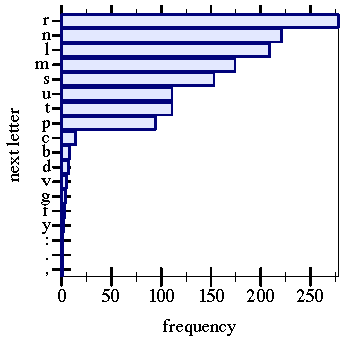
\includegraphics[trim=2.4000000000000004 2.4000000000000004 2.4000000000000004 2.4000000000000004]{pict.pdf}}}\end{FigureInside}\end{Centerfigure}

\Centertext{\Legend{\FigureTarget{\label{t:x28counter_x28x22figurex22_x22cax2dhistogramx22x29x29}Figure~1: }{t:x28counter_x28x22figurex22_x22cax2dhistogramx22x29x29}distribution of letters following\Scribtexttt{"ca"}}}\end{Figure}

In order to generate idiomatic text from this model, then,
we should observe these distributions. That is, if the last
two characters were \Scribtexttt{"ca"}, the next character should be
an \Scribtexttt{"r"} with probability 278/1397.

How should we make this choice? One way would be to draw
enough bits (11) from our pool to get a number larger than
1397, and then, say, pick the letter \Scribtexttt{"r"} if the number
is less than 278. Note, though, that while our program will
be deterministic (since it gets its randomness from the
stream of given bits), it will \textit{not} represent a
bijection, since (at least) 278 of the 2048 possible choices
all go to the same state.

To solve this, we need a way of drawing fewer bits to make
more common choices, and drawing more bits to make rarer
ones.

Fortunately, this is exactly the problem that Huffman trees solve!

\sectionNewpage

\Ssection{Huffman Trees}{Huffman Trees}\label{t:x28part_x22Huffmanx5fTreesx22x29}

Huffman trees~(Huffman and others 1952) are generally used in
compression. The basic idea is that we can build a binary
tree where more{-}common choices are close to the root, and
less{-}common choices are further from the root.

The standard construction algorithm for Huffman trees
proceeds by coalescing; starting with a set of leaves with
weights, we join together the two least{-}weighty leaves into
a branch whose weight is the sum of its children. We then
continue, until at last we{'}re left with just one tree.

As an example, we can consider the distribution given above.
In this case, there are several characters (the comma, the
period, and the colon) that occur just once.  We would
therefore combine two of these (the comma and the period,
say) into a branch with weight two and two children, the
comma and period leaves. Next, we would combine the colon
(the only tree left with weight one) with either the
\Scribtexttt{"y"} or the branch formed in the previous step; each has
weight two. The result would have weight three.

Proceeding in this way, we arrive at the tree shown in
figure~\FigureRef{2}{t:x28counter_x28x22figurex22_x22nextx2dletterx2dtreex22x29x29}.

\begin{Figure}\begin{Centerfigure}\begin{FigureInside}\raisebox{-0.6499999999999773bp}{\makebox[156.0bp][l]{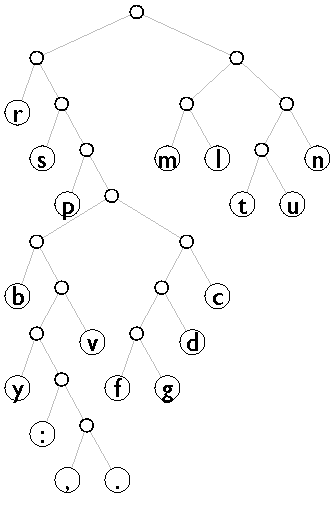
\includegraphics[trim=2.4000000000000004 2.4000000000000004 2.4000000000000004 2.4000000000000004]{pict_2.pdf}}}\end{FigureInside}\end{Centerfigure}

\Centertext{\Legend{\FigureTarget{\label{t:x28counter_x28x22figurex22_x22nextx2dletterx2dtreex22x29x29}Figure~2: }{t:x28counter_x28x22figurex22_x22nextx2dletterx2dtreex22x29x29}Huffman tree encoding next{-}letter choice from state \Scribtexttt{"ca"}}}\end{Figure}

If this tree were to be used in compression, we would
represent the transition to the letter \Scribtexttt{"r"} using two
bits, a zero and a zero (if we use zeros to denote left
branches). The transition to the next most likely letter,
\Scribtexttt{"l"}, would be represented as one{-}zero{-}one. Note that
less common choices are encoded using larger numbers of
bits.

We are not interested in compression, but in generation. For
this use case, we imagine that we are "decoding" the random
bit stream. So, for instance, if the random bit stream
contains the bits (0100110), we would use the first six bits
to reach the leaf \Scribtexttt{"c"}, and leave the remaining zero in
the stream.

Once we{'}ve reached a character, we may add this character to
the output stream. In order to continue, we must then start
again, in the new state.  If, for instance, the \Scribtexttt{"l"}
were chosen, we would now be in the state corresponding to
the letter pair \Scribtexttt{"al"}, and we would begin again.

Consider once more the problem of proving that this is a
bijection. In contrast to the earlier scheme, note that if
two bit streams differ first at (say) bit \relax{\(n\)}, then the
character that is output at that point in the model{'}s
operation is guaranteed to be different. This ensures that
each bit stream corresponds to a different output. To see
the other half of the bijection, we observe that given a
model{'}s output, we can simply run the "compression"
algorithm to obtain the sequence of bits that generated it.

\Ssubsection{Running Out of Bits}{Running Out of Bits}\label{t:x28part_x22Runningx5fOutx5fofx5fBitsx22x29}

One minor complication arises in that the given scheme is
not guaranteed to end "neatly". That is, the model may have
only partially traversed a huffman tree when the end of the
input bit stream is reached. We can easily solve this by
observing the bijection between streams of 56 randomly
generated bits and the infinite stream of bits whose first
56 bits are randomly generated and whose remaining bits are
all {``}zero{''}, in much the same way that an integer is not
changed by prepending an infinite stream of zeros. This
allows us to implement a bit generator that simply defaults
to {``}zero{''} when all bits are exhausted. In fact, the model
could continue generating text, but there{'}s no need to do
so, since the 56 random bits have already been used.

\Ssubsection{The Forbidden state}{The Forbidden state}\label{t:x28part_x22Thex5fForbiddenx5fstatex22x29}

Can our Markov model get stuck? This can occur if there is a
state with no outgoing transition. Fortunately, the
construction of the tree guarantees there will always be at
least one transition... except for the final characters
of the file. If this sequence occurs only once in the text
file, it{'}s conceivable that the model could get stuck. This
problem can easily be solved, though, by considering the source
document to be {``}circular,{''} and adding a transition from the
final state to the file{'}s initial character.

\Ssubsection{Choosing a Markov Model}{Choosing a Markov Model}\label{t:x28part_x22Choosingx5fax5fMarkovx5fModelx22x29}

In our examples thus far, we have chosen to use exactly two
characters as the states in the Markov model.  This is by no
means the only choice. We can easily use one character, or
three or four.

The tradeoff is fairly clear: using shorter
character{-}strings results in strings that sound less like
English, and using longer character{-}strings results in
strings that more like English. There is, however, a price;
the idiomaticity of the resulting strings results from a
lower "compression", measured in bits per character. That
is, the one{-}character markov model results in short strings,
and the three{-} and four{-}character models result in longer
ones. Naturally, all of the given models have the randomness
properties we{'}ve shown for the two{-}character ones, and users
may certainly choose a three{-} or four{-}character model, if
they find that the increase in memorability compensates for
the increase in length.

A final note concerns the selection of the initial state.
We{'}ve chosen to choose from those states starting with a
space, in order to simulate a password that begins "at the
beginning of a word," and we build a huffman tree to choose
from these initial states basen on their frequency within
the text.

\sectionNewpage

\Ssection{Examples}{Examples}\label{t:x28part_x22Examplesx22x29}

The proof is in the pudding! Let{'}s see some examples.

First, we generate strings using the one{-}character Markov model:

\begin{SingleColumn}\Scribtexttt{sochete ftr d f}

\Scribtexttt{walowemfronlo}

\Scribtexttt{them{-}l parof h o}

\Scribtexttt{tacupis anemas a}

\Scribtexttt{ar ps o hen tsefr}

\Scribtexttt{adowepr,{-}ce he T}

\Scribtexttt{land tr slor{\hbox{\texttt{.}}} ter}

\Scribtexttt{my lly af a sioo}\end{SingleColumn}

These may be seen to be short, but contain challenging
sequences, such as \Scribtexttt{lly af a}.

Next, strings generated using the two{-}character Markov model:

\begin{SingleColumn}\Scribtexttt{witaing her or to soma}

\Scribtexttt{ronstionsay ragao}

\Scribtexttt{wiliking hus ands this st}

\Scribtexttt{in{\hbox{\texttt{.}}}{\textquotesingle}s{\hbox{\texttt{.}}}{-}{-}overstichery}

\Scribtexttt{Driess, bursto anc}

\Scribtexttt{guavichfultakfull}

\Scribtexttt{way, Lounto coverb}

\Scribtexttt{Yah{\hbox{\texttt{!}}}{-}{-}by be wings,{-}{-}wi}\end{SingleColumn}

These are slightly longer, but much more pronounceable, and
appear somewhat more memorable.

Next, strings generated using the three{-}character Markov model:

\begin{SingleColumn}\Scribtexttt{younde; a mad revide s}

\Scribtexttt{thround eignal coff his, m}

\Scribtexttt{he who{\textquotesingle}s rests{\hbox{\texttt{.}}} The off}

\Scribtexttt{freets, Mr{\hbox{\texttt{.}}} Befolks our chr}

\Scribtexttt{not on the said Midn{\textquotesingle}t hest}

\Scribtexttt{of peak out it, an off (m}

\Scribtexttt{were walls{\hbox{\texttt{.}}} Twice that{\hbox{\texttt{.}}} It i}

\Scribtexttt{know thin one be thing; i}\end{SingleColumn}

These are far more English{-}like, with many actual words. As
a side note, the phrases generated here and in by the prior
two{-}character model appear almost archaic, with words like
"younde," "coff," and "hest". Naturally, these are longer
than the prior set.

Finally, strings generated using the four{-}character Markov model:

\begin{SingleColumn}\Scribtexttt{naughed, Who tall her o}

\Scribtexttt{in them forturbatious, who I knew p}

\Scribtexttt{Fancy{\hbox{\texttt{?}}} News of all{\hbox{\texttt{?}}} Two{\hbox{\texttt{.}}} If than}

\Scribtexttt{growing lumbent if thankle imp}

\Scribtexttt{commonsteady for heavy had hom}

\Scribtexttt{a luncher{\textquotesingle}s sacrificers was{\hbox{\texttt{.}}} T}

\Scribtexttt{kiss Manettle clothed them, beni}

\Scribtexttt{naminished{-}{-}this{\hbox{\texttt{.}}} What{\hbox{\texttt{?}}} Oh{\hbox{\texttt{!}}} It wi}\end{SingleColumn}

At this point, it{'}s starting to become clear what the source
is, and in some strings, Sydney Carton appears by name. In
addition, you get some fairly interesting neologisms{---}in
this case, {``}forturbatious.{''} It{'}s not a word, but maybe it
should be.

\begin{FigureMulti}\begin{Centerfigure}\begin{FigureInside}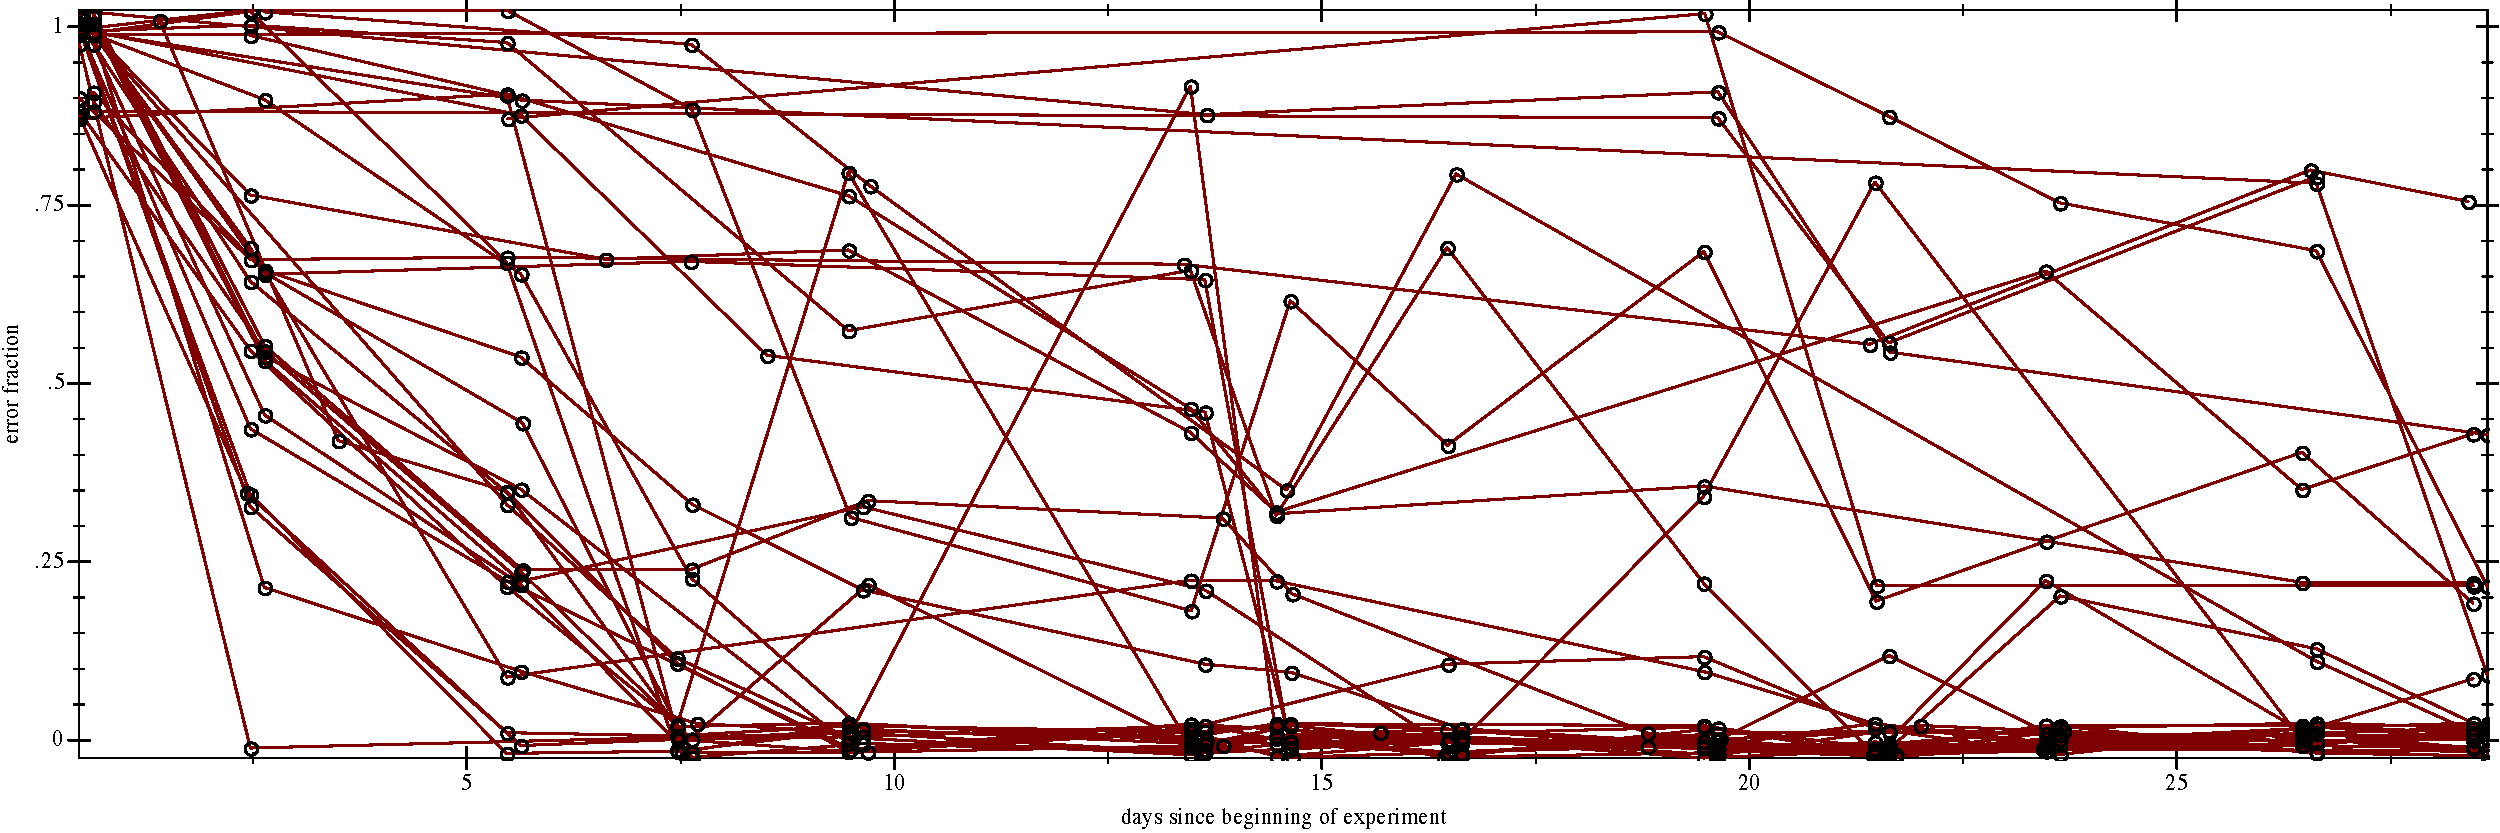
\includegraphics[scale=0.4]{control-group-sequences.pdf}\end{FigureInside}\end{Centerfigure}

\Centertext{\Legend{\FigureTarget{\label{t:x28counter_x28x22figurex22_x22controlx2dseqsx22x29x29}Figure~3: }{t:x28counter_x28x22figurex22_x22controlx2dseqsx22x29x29}performance of control group in first box}}\end{FigureMulti}

\begin{FigureMulti}\begin{Centerfigure}\begin{FigureInside}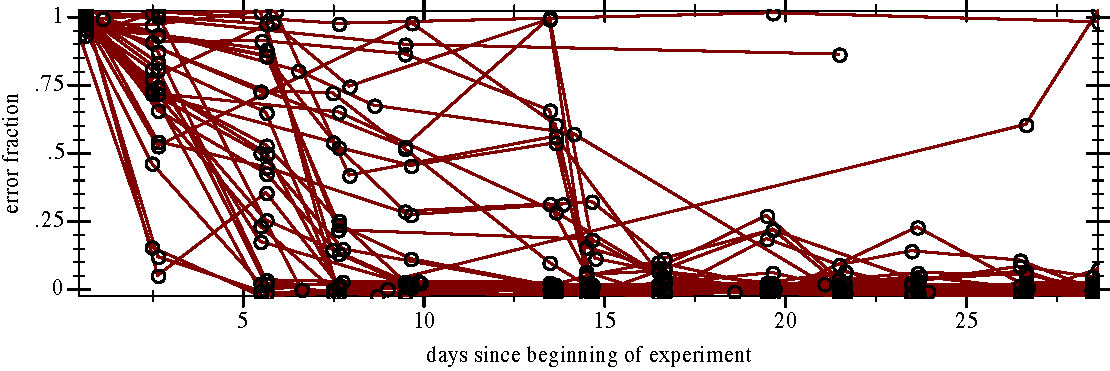
\includegraphics[scale=0.4]{experimental-group-sequences.pdf}\end{FigureInside}\end{Centerfigure}

\Centertext{\Legend{\FigureTarget{\label{t:x28counter_x28x22figurex22_x22experimentalx2dseqsx22x29x29}Figure~4: }{t:x28counter_x28x22figurex22_x22experimentalx2dseqsx22x29x29}performance of experimental group in first box}}\end{FigureMulti}

\sectionNewpage

\Ssection{Choice of Corpus}{Choice of Corpus}\label{t:x28part_x22Choicex5fofx5fCorpusx22x29}

Naturally, the choice of \textit{A Tale of Two Cities} is
largely arbitrary; any corpus of reasonable length will
suffice. One intriguing possibility would be to choose the
full text of all of the e{-}mails in a particular user{'}s
history.\NoteBox{\NoteContent{ This is actually not hypothetical; we do
exactly this in the generation of our own passwords.}} This
text would presumably reflect the style of text that a
particular user is accustomed to read and write, and should
in principle be extraordinarily memorable.  Note that the
security of the system is entirely independent of the chosen
corpus; our attack model assumes that the attacker already
has the full text of the corpus.

\sectionNewpage

\Ssection{Evaluation}{Evaluation}\label{t:x28part_x22Evaluationx22x29}

In order to explore the advantages of our proposed system,
we designed and executed an experiment.

\Ssubsection{Subjects and Procedure}{Subjects and Procedure}\label{t:x28part_x22Subjectsx5fandx5fProcedurex22x29}

Specifically, we recruited students from an upper{-}level
university class to participate in a one{-}minute training
session at the beginning of an in{-}class lab, each time it
met. These sessions occurred three times a week, and the
experiment ran for a total of 13 sessions. The students were
randomly assigned to either the experimental group or to the
control group.  Each student was assigned a single password
to be learned during the course of the experiment. Those in
the experimental group were assigned a password generated
using our system, set to use an order{-}two model generated
from \textit{A Tale of Two Cities}. Those in the control group
were assigned a random nine{-} or ten{-}character password
generated by choosing randomly from a set of characters.
Both the experimental and the control passwords were
generated using 56 bits of randomness each.

At the beginning of each lab session, students visited a web
page that required them to log in using existing student
credentials, and then asked them to type the password that
they{'}d been given. (Naturally, the first time they used the
system, their guesses were blank.) Following this, they were
shown the correct password and asked to type it three times
with the assistance of green and red squares indicating
whether the corresponding character had been typed
correctly.

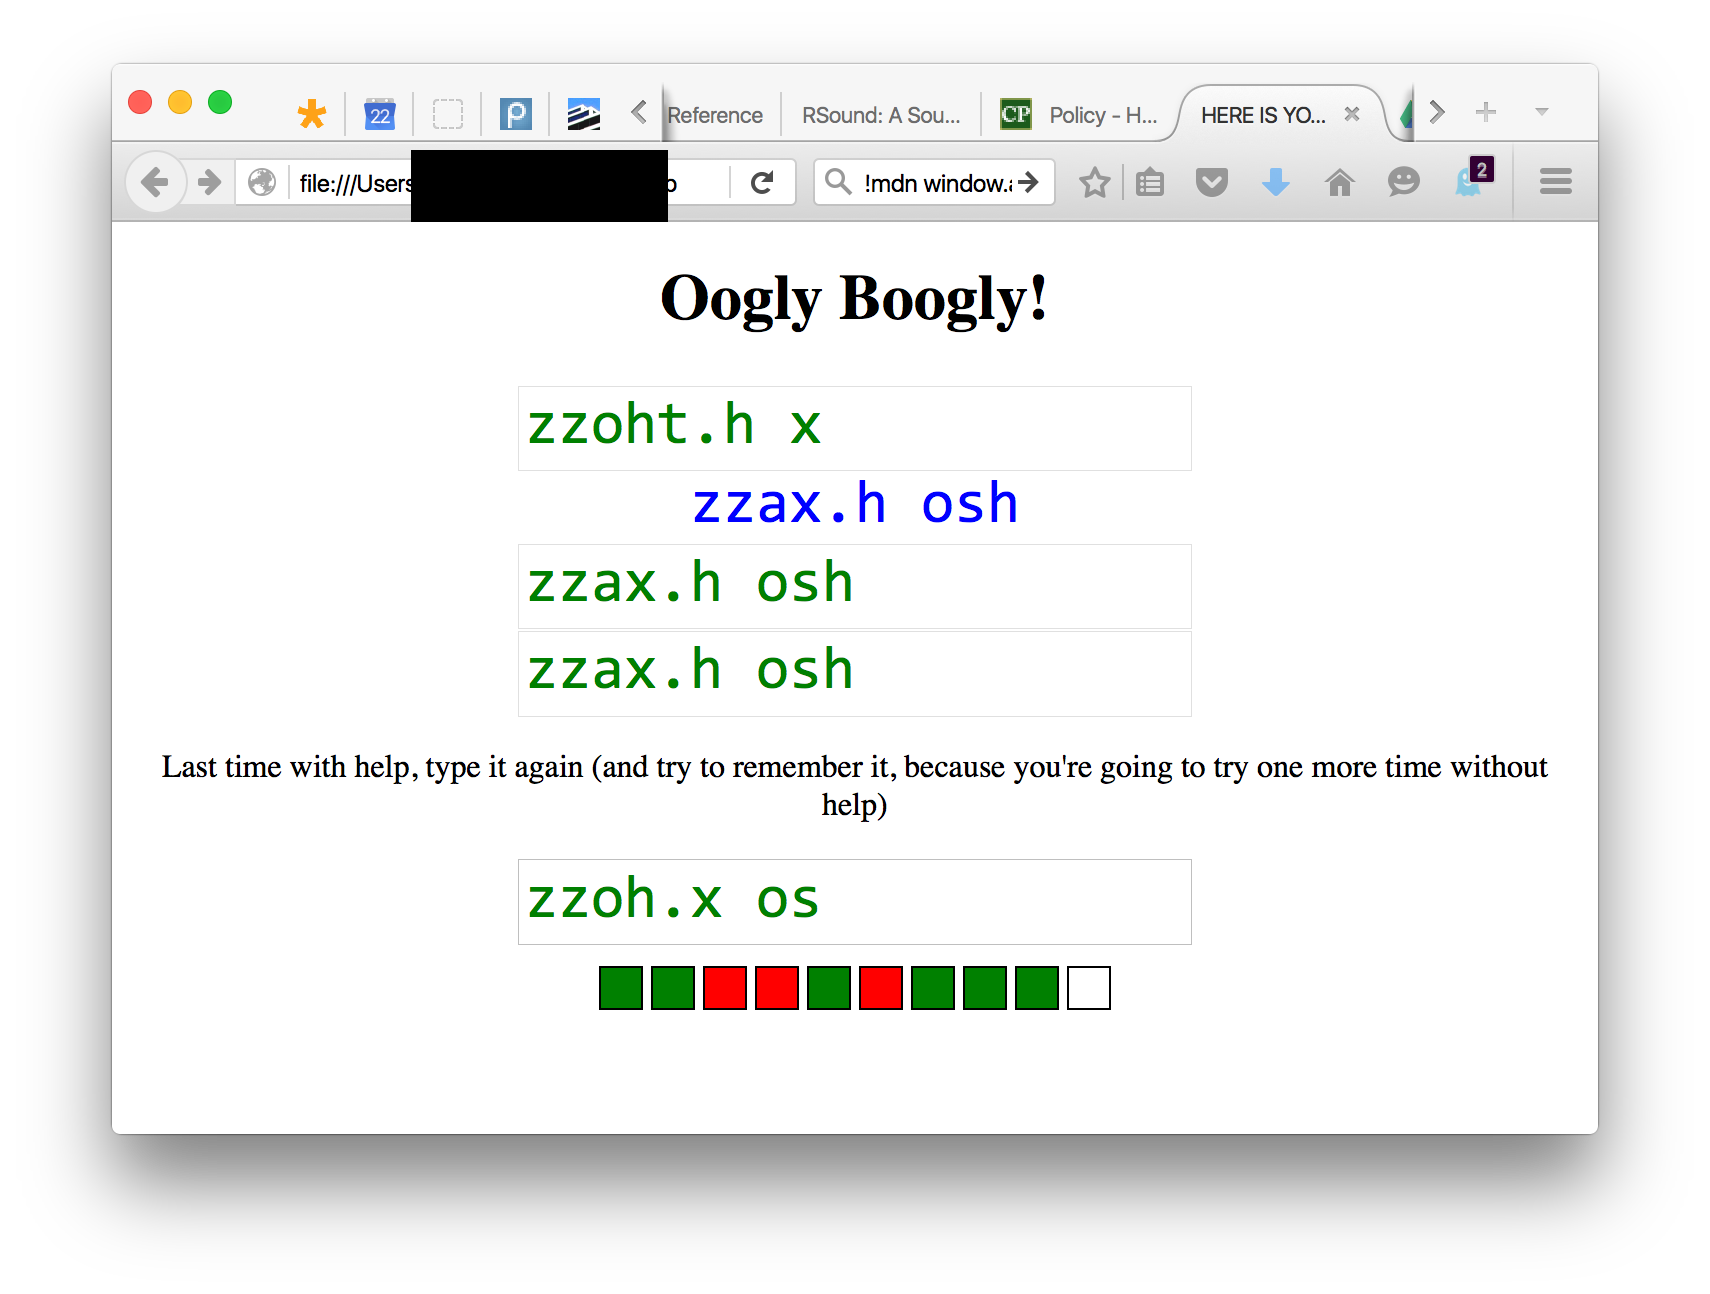
\includegraphics[scale=0.27]{screenshot.png}

After three assisted attempts, students were again
challenged to type the password without being able to see
it. They were then finished, until the next training
session.

During the student{'}s interaction, the system logged each
users{'}s session start, and every change to a password entry
box, along with timing information. In essence, the system
acted as a keylogger.

Note that no active deception was involved in the
experiment; students knew that they were participating in a
study about the memorability of passwords. The experiment{'}s
plan was reviewed by our institution{'}s Human Subjects review
panel, and deemed {``}exempt from further review.{''}

\Ssubsection{Pre{-}Registration}{Pre{-}Registration}\label{t:x28part_x22Prex2dRegistrationx22x29}

While the experiment was going on, we discovered the
existence of the Open Science Foundation, online at
\href{http://osf.io/}{\Snolinkurl{http://osf.io/}}. Their mission is to help ensure the
quality of experimentation in the natural sciences by
allowing experimenters to describe the experiments that they
are performing and the analyses that they plan to perform
\textit{before} examining the data and extracting the
hypotheses that are best supported by the data ({``}hmm, it
looks like passwords containing exactly three spaces are
much more memorable!{''}). We registered our project,
providing pointers to code, and a plan for analysis
~(Bogus 2097).

In our pre{-}registration, we described two hypotheses. The
first was that our passwords would be learned more quickly,
and the second was that they would be retained longer.

Additionally, we decided to omit the information of any student
that participated fewer than three times.

\Ssubsection{Analysis}{Analysis}\label{t:x28part_x22Analysisx22x29}

In order to measure password learning, our primary
instrument was the password entered by each student into the
first, unprompted, password box that was a part of each
session. We used Levenshtein string distance
~(Bogus 2097) as a measure of password
correctness. This metric measures the number of
one{-}character changes{---}insertions, deletions, or
substitutions{---}that are necessary to change one string into
another. So, for instance, if the student omitted one
character and replaced an {`}a{'} with an {`}e{'} but was otherwise
correct, the Levenshtein distance would be computed as two.
We then divided this by the number of characters in the
password to obtain a measure of error that ranges from 0,
representing a correct password entry, to 1.0, representing
an entirely wrong password.

Figure~\FigureRef{3}{t:x28counter_x28x22figurex22_x22controlx2dseqsx22x29x29} shows the behavior of the
students in the control group in the first box from each
day{'}s training. Figure~\FigureRef{4}{t:x28counter_x28x22figurex22_x22experimentalx2dseqsx22x29x29} shows the behavior of the students in
the experimental group in the first box from each day{'}s
training. Each point corresponds to a single student{'}s
session. In these graphs, each error value was perturbed by
a random value in the range \relax{\((-0.025,0.025)\)}, in order to
prevent the preponderance of points precisely on the x axis
from all obscuring each other.

A quick glance at these two figures suggests that there is in
fact a difference between the two groups. But is it the difference
that we hypothesized?

\Ssubsubsection{Not Really, No}{Not Really, No}\label{t:x28part_x22Notx5fReallyx5fx5fNox22x29}

Our first hypothesis was that the experimental passwords
would be learned more quickly than the control passwords.

In order to measure this, we fitted a simple two{-}part linear
model to each student{'}s performance. The model is parameterized
by a single parameter, a {``}learning time,{''} \relax{\(l\)}. The model
is then defined by the functions \relax{\(f_l\)}:

\relax{\[f_l(t) =
\left\{
  \begin{array}{lr}
    1 - t/l & $when $ t<l \\
    0 & $otherwise$
  \end{array}
\right.\]}

For each student, we chose the value of \relax{\(l\)} that minimized the
mean{-}square distance between the sample points and the fitted line.

\begin{Figure}\begin{Centerfigure}\begin{FigureInside}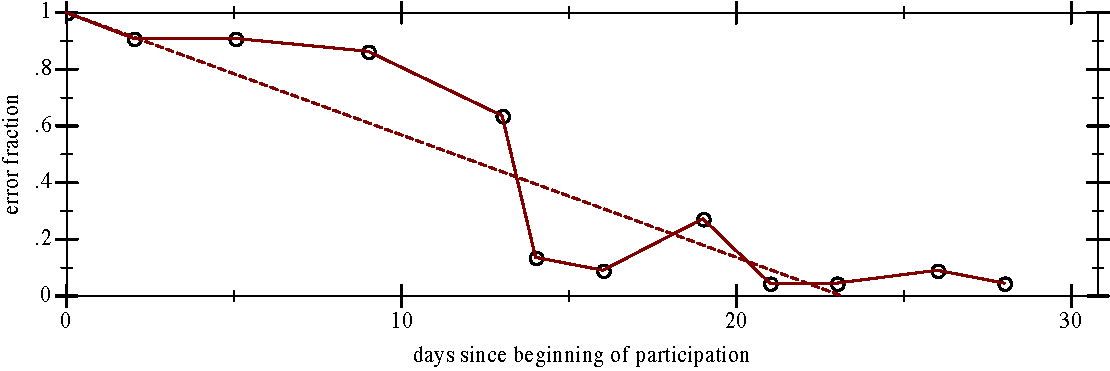
\includegraphics[scale=0.2]{best-fit-1.pdf}
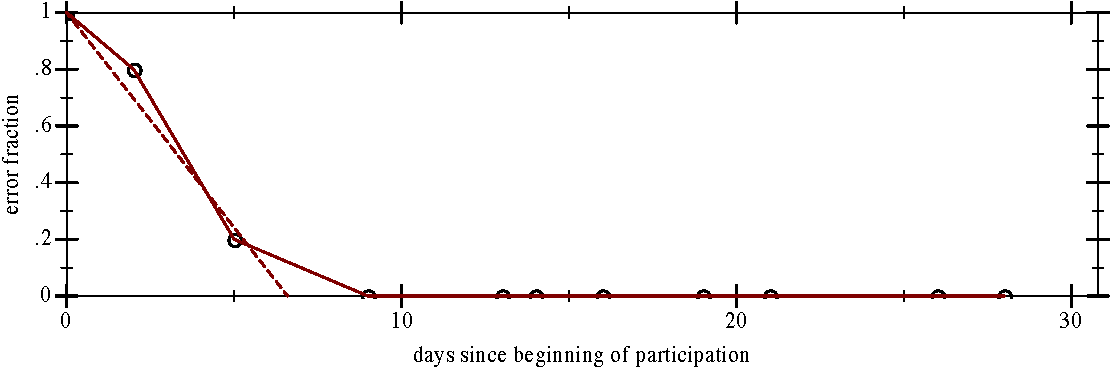
\includegraphics[scale=0.2]{best-fit-2.pdf}
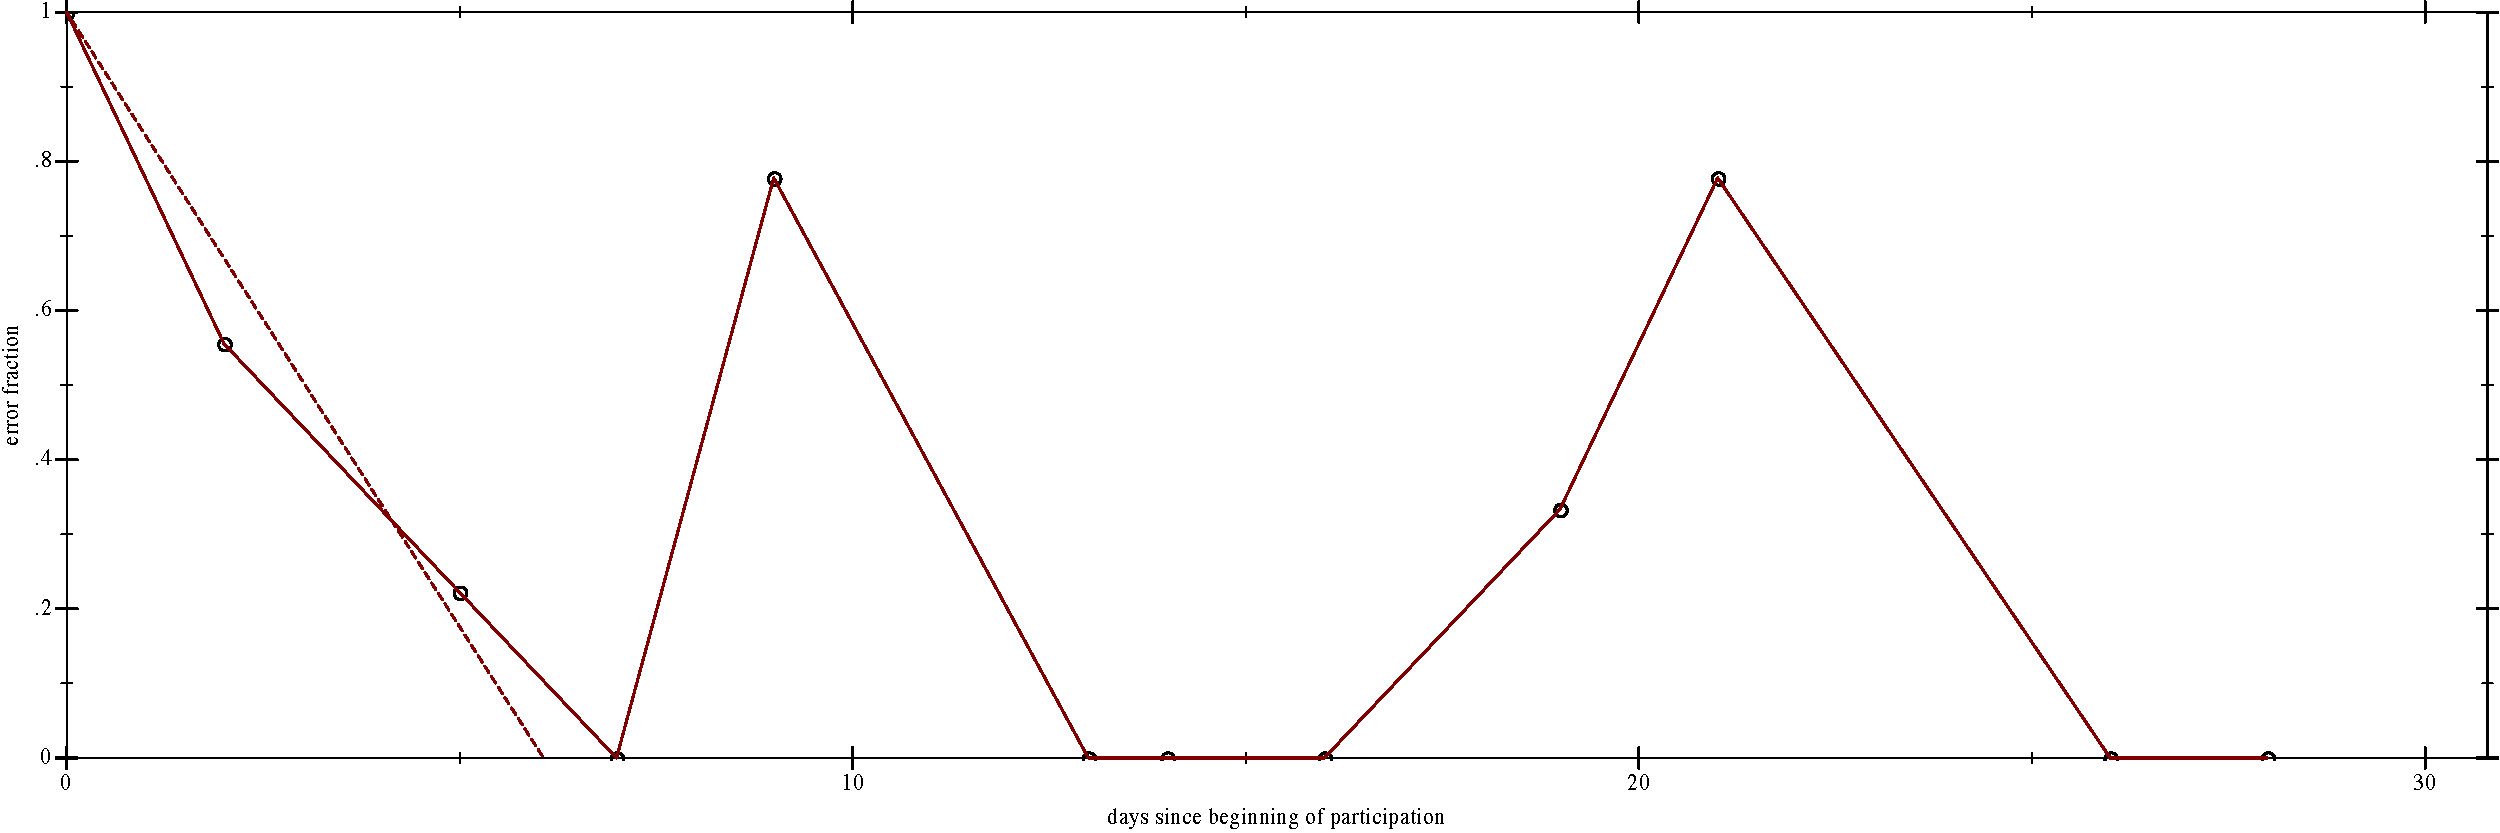
\includegraphics[scale=0.2]{best-fit-4.pdf}\end{FigureInside}\end{Centerfigure}

\Centertext{\Legend{\FigureTarget{\label{t:x28counter_x28x22figurex22_x22bestx2dfitsx22x29x29}Figure~5: }{t:x28counter_x28x22figurex22_x22bestx2dfitsx22x29x29}student traces and best{-}fit model for three students}}\end{Figure}

Figure~\FigureRef{5}{t:x28counter_x28x22figurex22_x22bestx2dfitsx22x29x29} shows examples of the best{-}fit model for
three different students. The first one learns slowly, with an estimated
time of about 23 days to learn. The second (more typical) one learns
quickly, with an estimated time of about 6.5 days to learn. The third
one illustrates one of the problems with the model; the best fit shows
that learning took 6 days, despite clear problems in recall in later
experiments.

\begin{FigureMulti}\begin{Centerfigure}\begin{FigureInside}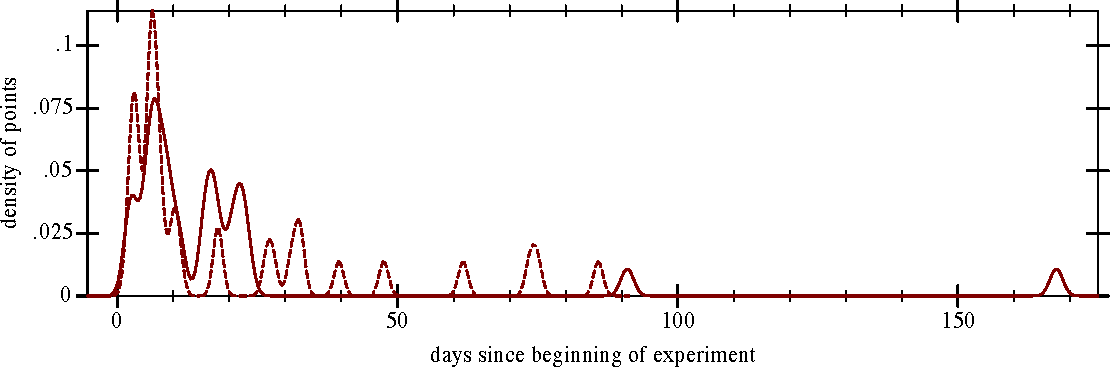
\includegraphics[scale=0.4]{time-to-learn.pdf}\end{FigureInside}\end{Centerfigure}

\Centertext{\Legend{\FigureTarget{\label{t:x28counter_x28x22figurex22_x22timex2dtox2dlearnx22x29x29}Figure~6: }{t:x28counter_x28x22figurex22_x22timex2dtox2dlearnx22x29x29}estimated learning times (control group dashed lines)}}\end{FigureMulti}

Noisy data notwithstanding, we computed a value of \relax{\(l\)} for each
member of the control and experimental group. Figure~\FigureRef{6}{t:x28counter_x28x22figurex22_x22timex2dtox2dlearnx22x29x29}
graphs the density of the values of \relax{\(l\)} for each group. That is, we
convolve a graph of impulse functions with normal kernels to show a
"smoothed" density graph. Each group{'}s density curve has an integral
of 1.\NoteBox{\NoteContent{We adopt this alternative to a histogram in order to avoid
the inevitable bias that occurs as a result of the selection of bin
boundaries.}} The control group is shown as a dashed line.

Omitted from this graph is one subject who entered his or her password
incorrectly with perfect consistency, leading to an estimated learning
time of infinity.\NoteBox{\NoteContent{Or, more precisely, to divergence of our
estimation algorithm.}}

Next, note the scale of the \relax{\(x\)} axis; The experiment lasted for
28 days, and the rightmost entry on this density graph lies at about 168
days.

Our first observation is that the two sets are not normally distributed
by any stretch of the imagination. Attempting to perform a student{'}s
t{-}test, for instance, would be relatively meaningless. Each one has
a remarkably strong density in the five{-}to{-}six day range, with a number
of outliers.
Specifically, approximately one sixth of the participants have values
of \relax{\(l\)} greater than 28 days, the length of the experiment,
indicating essentially that they do not
appear to have learned their passwords.

Next, inspection suggests that many of the outliers are students that
participated in a relatively small number of trials. Naturally, we
would expect these students to take longer to learn their passwords.

Can we conclude that students learn the experimental passwords more
quickly? No, we cannot. Both distributions appear to have a heavy
tail, and in fact, the control group has a stronger representation
among the very quickest learners.

\Ssubsubsection{Retention}{Retention}\label{t:x28part_x22Retentionx22x29}

Our second stated hypotheses was that students would retain their
passwords better in the experimental group. The final piece of this
experiment is a delay of two weeks, after which the students will
be asked (in the context of the class final exam) to produce their
password (on an anonymous slip of paper). This will provide a measure
of password retention. As a side benefit, it may also help to identify
those that were cheating by recording their password in digital form.

\Ssubsection{Data Mining}{Data Mining}\label{t:x28part_x22Datax5fMiningx22x29}

Building post{-}hoc hypotheses is a big no{-}no. This is called {``}p{-}hacking,{''}
based on the observation that for a given set of data, it is nearly
always possible to tweak and grind the hypothesis in order to obtain
statistical significance.

What follows, then, is not a test of a hypothesis, but rather simply
a set of observations that might lead to further hypotheses.

\begin{FigureMulti}\begin{Centerfigure}\begin{FigureInside}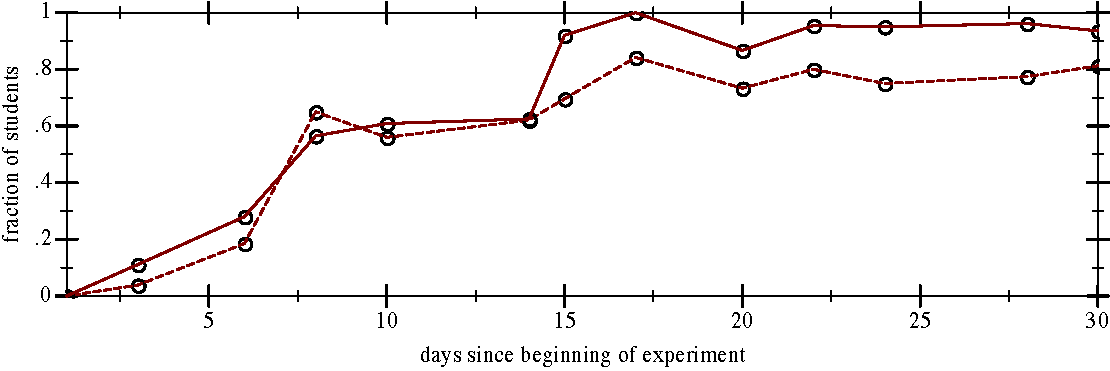
\includegraphics[scale=0.4]{pct-below-20-thresh.pdf}\end{FigureInside}\end{Centerfigure}

\Centertext{\Legend{\FigureTarget{\label{t:x28counter_x28x22figurex22_x2220x2dpercentx2derrorx22x29x29}Figure~7: }{t:x28counter_x28x22figurex22_x2220x2dpercentx2derrorx22x29x29}fraction of students with less than 20\% error (control dashed)}}\end{FigureMulti}

Our inspection of the graphs in figure~\FigureRef{3}{t:x28counter_x28x22figurex22_x22controlx2dseqsx22x29x29} and
figure~\FigureRef{4}{t:x28counter_x28x22figurex22_x22experimentalx2dseqsx22x29x29}, along with our analysis of estimated
learning times, suggests that the control group contains a substantial
subgroup that has not learned their passwords at all. In order to
measure this, we graphed, for various error levels, the fraction
of students in each session whose error was below the specified
level. Figure~\FigureRef{7}{t:x28counter_x28x22figurex22_x2220x2dpercentx2derrorx22x29x29} shows the fraction of students
that had an error level of less than 20\% in a given test. As before,
the dashed line indicates the control group.

In this graph, it appears that a significantly larger fraction of the
students in the experimental group recalled their passwords, but only
after an initial learning period of approximately 6 sessions.
The graphs for 10\%, 30\%, and 40\% are similar. It would be relatively
straightforward to attempt to validate this with a second experiment
that focuses on this aspect of the project.

\Ssubsection{Threats to Validity}{Threats to Validity}\label{t:x28part_x22Threatsx5ftox5fValidityx22x29}

Naturally, any study with live subjects is subject to threats to validity
both internal and external.

One potential internal threat to validity arises as a result of possible
cheating. It its certainly possible for students to copy and paste the
passwords from the web page. We do not see much evidence of this, both
in that only one student appears to have learned the password after one
session, and also in that our keystroke data shows only one instance in
which the password "appeared" in exactly one keystroke. Additionally,
we see no reason to expect the experimental group to cheat more than
the control group, or vice versa.

\Ssubsection{Cheating}{Cheating}\label{t:x28part_x22Cheatingx22x29}

The reader may wonder, at this point, whether the students
cheated. Certainly, they could have copied the web page from
the prompt, and memorized it offline, or simply pasted it
into place. In our

However, we saw little evidence of this. The students
participated in a lab setting, which may have inclined them
toward honesty. Also, no course credit was associated with
performance in the experiment.

Finally, we believe that cheating{---}if it occurred{---}would
be equally likely among the control and experimental group.

\sectionNewpage

\Ssection{Reproducibility}{Reproducibility}\label{t:x28part_x22Reproducibilityx22x29}

We have made every effort to ensure that our work is
entirely reproducible, making available all code involved in
password generation and experimentation, and also the raw
(anonymized) data collected during the experiment.

FIXME urls here!

\sectionNewpage

\Ssection{Related Work}{Related Work}\label{t:x28part_x22Relatedx5fWorkx22x29}

There are many, many works that describe passwords. We have
cited Bonneau{'}s work before, and we will do so again here,
as this work was enormously informative~(Bonneau and Schechter 2014). We
have also already described the work contained in many other
related projects~(Leonhard and Venkatakrishnan 2007; NIST 1993).

To our knowledge, however, there is no other work that uses
a bit source to drive huffman decoding to drive a markov
model, thereby enabling generation of pronounceable text
without the (heretofore) attendant lack of
equi{-}probability.

\sectionNewpage

\Ssection{Future Work}{Future Work}\label{t:x28part_x22Futurex5fWorkx22x29}

FIXME

\sectionNewpage

\Ssection{Acknowledgments}{Acknowledgments}\label{t:x28part_x22Acknowledgmentsx22x29}

Many thanks to Zachary Peterson for instantly pinpointing
relevant research. Many thanks to Racket for being an
amazing programming language.

\sectionNewpage

\Ssectionstarx{Bibliography}{Bibliography}\label{t:x28part_x22docx2dbibliographyx22x29}

\begin{AutoBibliography}\begin{SingleColumn}\label{t:x28autobib_x22Anne_Adamsx2c_Martina_Angela_Sassex2c_and_Peter_LuntMaking_passwords_secure_and_usableIn_Procx2e_People_and_Computers_XIIx2c_ppx2e_1x2dx2d191997x22x29}\Autobibentry{Anne Adams, Martina Angela Sasse, and Peter Lunt. Making passwords secure and usable. In \textit{Proc. People and Computers XII}, pp. 1{--}19, 1997.}

\label{t:x28autobib_x22Bobby_BogusFIXMEAdd_a_real_reference_herex2ex2ex2e2097x22x29}\Autobibentry{Bobby Bogus. FIXME. Add a real reference here..., 2097.}

\label{t:x28autobib_x22Joseph_BonneauThe_science_of_guessingx3a_analyzing_an_anonymized_corpus_of_70_million_passwordsIn_Procx2e_2012_IEEE_Symposium_on_Security_and_Privacy2012x22x29}\Autobibentry{Joseph Bonneau. The science of guessing: analyzing an anonymized corpus of 70 million passwords. In \textit{Proc. 2012 IEEE Symposium on Security and Privacy}, 2012.}

\label{t:x28autobib_x22Joseph_Bonneau_and_Stuart_SchechterTowards_reliable_storage_of_56x2dbit_secrets_in_human_memoryIn_Procx2e_Procx2e_USENIX_Security2014x22x29}\Autobibentry{Joseph Bonneau and Stuart Schechter. Towards reliable storage of 56{-}bit secrets in human memory. In \textit{Proc. Proc. USENIX Security}, 2014.}

\label{t:x28autobib_x22Nicholas_Jx2e_Cepedax2c_Harold_Pashlerx2c_Edward_Vulx2c_John_Tx2e_Wixtedx2c_and_Doug_RohrerDistributed_practice_in_verbal_recall_tasksx3a_A_review_and_quantitative_synthesisPsychological_Bulletin_132x283x292006x22x29}\Autobibentry{Nicholas J. Cepeda, Harold Pashler, Edward Vul, John T. Wixted, and Doug Rohrer. Distributed practice in verbal recall tasks: A review and quantitative synthesis. \textit{Psychological Bulletin} 132(3), 2006.}

\label{t:x28autobib_x22Charles_DickensA_Tale_of_Two_CitiesChapman_x26_Hall1859x22x29}\Autobibentry{Charles Dickens. A Tale of Two Cities. Chapman \& Hall, 1859.}

\label{t:x28autobib_x22Hermann_Ebbinghausxdcber_das_gedxe4chtnisx3a_untersuchungen_zur_experimentellen_psychologieDuncker_x26_Humblot1885x22x29}\Autobibentry{Hermann Ebbinghaus. \"{U}ber das ged\"{a}chtnis: untersuchungen zur experimentellen psychologie. Duncker \& Humblot, 1885.}

\label{t:x28autobib_x22Ravi_Ganesan_and_Chris_DaviesA_new_attack_on_random_pronounceable_password_generatorsIn_Procx2e_Proceedings_of_the_17th_NISTx2dNCSC_National_Computer_Security_Conference1994x22x29}\Autobibentry{Ravi Ganesan and Chris Davies. A new attack on random pronounceable password generators. In \textit{Proc. Proceedings of the 17th NIST{-}NCSC National Computer Security Conference}, 1994.}

\label{t:x28autobib_x22David_Ax2e_Huffman_and_othersA_method_for_the_construction_of_minimum_redundancy_codesProceedings_of_the_IRE_40x289x29x2c_ppx2e_1098x2dx2d11011952x22x29}\Autobibentry{David A. Huffman and others. A method for the construction of minimum redundancy codes. \textit{Proceedings of the IRE} 40(9), pp. 1098{--}1101, 1952.}

\label{t:x28autobib_x22Michael_Dx2e_Leonhard_and_VN_VenkatakrishnanA_comparative_study_of_three_random_password_generatorsIEEE_EITx2c_ppx2e_227x2dx2d2322007x22x29}\Autobibentry{Michael D. Leonhard and VN Venkatakrishnan. A comparative study of three random password generators. \textit{IEEE EIT}, pp. 227{--}232, 2007.}

\label{t:x28autobib_x22Randall_MonroePassword_Strengthx2c_XKCD_x23936on_the_webx3a_httpx3ax2fx2fwwwx2exkcdx2ecomx2f936x2f2011x22x29}\Autobibentry{Randall Monroe. Password Strength, XKCD \#936. on the web: http://www.xkcd.com/936/, 2011.}

\label{t:x28autobib_x22NISTAutomated_Password_GeneratorFederal_Information_Processing_Standards_Publication_Nox2e_1811993x22x29}\Autobibentry{NIST. Automated Password Generator. Federal Information Processing Standards Publication No. 181, 1993.}

\label{t:x28autobib_x22Claude_Ex2e_ShannonA_Mathematical_Theory_of_CommunicationBell_System_Technical_Journal_7x2c_ppx2e_379x2dx2d4231948x22x29}\Autobibentry{Claude E. Shannon. A Mathematical Theory of Communication. \textit{Bell System Technical Journal} 7, pp. 379{--}423, 1948.}

\label{t:x28autobib_x22Chris_StreetRIDYHEWx2e_The_RIDiculouslY_Huge_English_Wordliston_the_webx3a_httpx3ax2fx2fwwwx2ecodehappyx2enetx2fwordlistx2ehtmx22x29}\Autobibentry{Chris Street. RIDYHEW. The RIDiculouslY Huge English Wordlist. on the web: http://www.codehappy.net/wordlist.htm.}\end{SingleColumn}\end{AutoBibliography}

\postDoc
\end{document}
